% !TEX TS-program = arara
% arara: xelatex: { synctex: on, options: '-halt-on-error'}
% arara: biber
% skip-arara: makeglossaries
% skip-arara: makeindex
% arara: xelatex: { synctex: on, options: '-halt-on-error'}
% arara: xelatex: { synctex: on, options: '-halt-on-error'}
% arara: clean: { files: [ overview.aux, overview.bbl] }
% arara: clean: { files: [ overview.bcf, overview.blg] }
% arara: clean: { files: [ overview.glg, overview.glo] }
% arara: clean: { files: [ overview.gls, overview.gls] }
% arara: clean: { files: [ overview.idx, overview.ilg] }
% arara: clean: { files: [ overview.ind, overview.loe] }
% arara: clean: { files: [ overview.lof, overview.log ] }
% arara: clean: { files: [ overview.log, overview.lol ] }
% arara: clean: { files: [ overview.out ] }
% arara: clean: { files: [ overview.run.xml] }
% arara: clean: { files: [ overview.toc, overview.xdy] }
% arara: clean: { files: [ overview.synctex.gz] }
%-----------------------------------------------------------------
\documentclass[10pt,openany]{article}
\errorcontextlines 10000
%-------------------------------------------------------------------------------
% layout file determines 1/2 col, landscape/portrait...
\usepackage{geometry}
%-------------------------------------------------------------------------------
\usepackage{color}
\usepackage[dvipsnames,svgnames,x11names]{xcolor}
%-------------------------------------------------------------------------------
\usepackage{graphics}
\usepackage{epsfig}
\usepackage{graphicx}
\PassOptionsToPackage{normalem}{ulem}
\usepackage{ulem}
%-------------------------------------------------------------------------------
\usepackage{url}
%-------------------------------------------------------------------------------
\usepackage[english]{babel}
%-------------------------------------------------------------------------------
\usepackage{csquotes}
%-------------------------------------------------------------------------------
\usepackage{epigraph}
\setlength{\epigraphwidth}{\linewidth}
%-------------------------------------------------------------------------------
\usepackage{fontspec}
%-------------------------------------------------------------------------------
% http://www.georgduffner.at/ebgaramond/download.html
% https://bitbucket.org/georgd/eb-garamond/downloads/EBGaramond-0.016.zip
\IfFontExistsTF{EB Garamond}{\message{---EB Garamond---}
  \fontspec[SmallCapsFeatures={Letters=SmallCaps},]{EB Garamond}
  \setmainfont[
    Path,
    UprightFont = *12-Regular,
    ItalicFont  = *12-Italic,
    BoldFont    = *08-Regular,
    BoldItalicFont = *08-Italic ]
    {EBGaramond}}
  {% https://www.microsoft.com/typography/fonts/family.aspx?FID=134
  \IfFontExistsTF{Garamond}{%
    \message{---Garamond---}
    \fontspec[SmallCapsFeatures={Letters=SmallCaps},]{Garamond}
    \setmainfont{Garamond}}
    {
    \IfFontExistsTF{Apple Garamond}{%
      \message{Apple Garamond}
      \setmainfont{Apple Garamond}}
      {\message{default main font}}}}

%\setmainfont{Palatino Linotype}
%\setmainfont{Perpetua}[Scale=1.1]
%\setmainfont{Times New Roman}
%-------------------------------------------------------------------------------
% https://www.microsoft.com/typography/fonts/family.aspx?FID=155
\IfFontExistsTF{Gill Sans MT}{%
  \message{---Gill Sans MT---}%
  \setsansfont{Gill Sans MT}}%
  {% http://arkandis.tuxfamily.org/adffonts.html
  \IfFontExistsTF{Gillius ADF}{%
    \message{---Gillius ADF---}%
    \setsansfont{Gillius ADF}}%
    \IfFontExistsTF{Gill Sans}{%
      \message{---Apple Gill Sans---}%
      \setsansfont{Gill Sans}}%
      {\message{---default Sans---}}}
%-------------------------------------------------------------------------------
% \setmonofont{}
%-------------------------------------------------------------------------------
% \usepackage{xeCJK}
% \setCJKmainfont{SimHei}
% \setCJKsansfont{SimHei}
% \setCJKmonofont{Lucida Sans Typewriter}
%-------------------------------------------------------------------------------
\usepackage{amsmath}
\usepackage{amssymb}
\DeclareMathOperator*{\argmin}{argmin}
\DeclareMathOperator*{\argmax}{argmax}
%\DeclareMathOperator*{\cdf}{cdf}
%\DeclareMathOperator*{\quantile}{quantile}
\newcommand\bigforall{\mbox{\Large $\mathsurround0pt\forall$}} 
%-------------------------------------------------------------------------------
\usepackage{amsthm}
%\theoremstyle{definition}
%\newtheorem{example}{Example}[section]
\usepackage{thmtools}
\theoremstyle{definition}
\DeclareRobustCommand{\rvspace}[1]{\vspace{#1}}
\declaretheoremstyle[
spaceabove=12pt,
spacebelow=10pt,
headpunct={\sffamily\mdseries:},
%headformat=margin,
headpunct={},
headfont=\sffamily\mdseries,
notefont=\sffamily\mdseries,
notebraces={}{},
bodyfont=\normalfont,
postheadspace=\newline,%
]{mythmstyle}
\declaretheorem[style=mythmstyle,title=Definition,name={Definition}]{definition}
\declaretheorem[style=mythmstyle,title=Example,name={Example}]{example}
\renewcommand{\thmtformatoptarg}[1]{#1}%
%-------------------------------------------------------------------------------
\numberwithin{definition}{subsection}
\numberwithin{example}{subsection}
\numberwithin{equation}{subsection}
\numberwithin{figure}{subsection}
%-------------------------------------------------------------------------------
\usepackage{listings}
\lstset{backgroundcolor={\color{GhostWhite}},
basicstyle={\ttfamily\small},
breaklines=false,
captionpos=b,
%frame=tblr,
mathescape=true,
escapechar=\%,
keywordstyle={\ttfamily}}
\renewcommand{\lstlistingname}{Listing}
\providecommand{\algorithmname}{Algorithm}
\providecommand{\exercisename}{Exercise}
\providecommand{\theoremname}{Theorem}
\providecommand{\examplename}{Example}
%-------------------------------------------------------------------------------
% \makeatletter
% \let\orig@item\item
% 
% \def\item{%
%     \@ifnextchar{[}%
%         {\lstinline@item}%
%         {\orig@item}%
% }
% 
% \begingroup
% \catcode`\]=\active
% \gdef\lstinline@item[{%
%     \setbox0\hbox\bgroup
%         \catcode`\]=\active
%         \let]\lstinline@item@end
% }
% \endgroup
% 
% \def\lstinline@item@end{%
%     \egroup
%     \orig@item[\usebox0]%
% }
% \makeatother
%-------------------------------------------------------------------------------
\usepackage{algpseudocode,algorithm,algorithmicx}
%-------------------------------------------------------------------------------
\usepackage{datetime}
\renewcommand{\dateseparator}{-}
\renewcommand{\today}{
\the\year \dateseparator \twodigit\month \dateseparator \twodigit\day}
%-------------------------------------------------------------------------------
\setlength{\parskip}{3pt}
\setlength{\parindent}{0pt}
\usepackage[parfill]{parskip}
%-------------------------------------------------------------------------------
% \usepackage{fancyhdr}
% \pagestyle{fancy}
% \setlength{\headwidth}{\textheight}
% \addtolength{\headwidth}{\columnsep}
% %\addtolength{\headwidth}{\marginparsep}
% %\addtolength{\headwidth}{\marginparwidth}
% \fancypagestyle{plain}{
% \fancyhead{} % clear all head fields 
% \fancyfoot{} % clear all foot fields
% \fancyfoot[RO,LE]{\textsf{\thepage}} 
% \fancyfoot[RE,LO]{\textsf{Draft of \today}}
% \renewcommand{\headrulewidth}{0.0pt}
% \renewcommand{\footrulewidth}{0.1pt}}
% \pagestyle{plain}
%-------------------------------------------------------------------------------
\usepackage{titling}
%\newfontfamily\titlefont[Scale=MatchUppercase]{Gill Sans MT}
%\renewcommand{\maketitlehooka}{\titlefont}
\pretitle{\begin{flushright}\Huge\sffamily\bfseries}
\posttitle{\par\end{flushright}\vskip 0.25em}
\preauthor{\begin{flushright}\sffamily\scshape\mdseries}
\postauthor{\par\end{flushright}}
\predate{\begin{flushright}\sffamily\scshape\mdseries}
\postdate{\par\end{flushright}}
%\setlength{\droptitle}{-80pt}
%-------------------------------------------------------------------------------
\usepackage[sf,small,compact]{titlesec}
%\newfontfamily\headingfont[]{New Yorker}
%\newfontfamily\headingfont[Scale=MatchUppercase]{Libre Caslon Display}
%\newfontfamily\headingfont[]{Perpetua Titling MT}
%\newfontfamily\headingfont[Scale=MatchUppercase]{Gill Sans MT}
%\newfontfamily\headingfont[Scale=MatchUppercase]{Gillius ADF}

\titleformat{\part}{\huge\sffamily\bfseries}{\thepart}{0.5em}{}
\titleformat{\chapter}{\LARGE\sffamily\bfseries}{\thechapter}{0.5em}{}
\titleformat{\section}{\Large\sffamily\bfseries}{\thesection}{0.5em}{}
\titleformat{\subsection}{\large\sffamily\bfseries}{\thesubsection}{0.5em}{}
\titleformat{\subsubsection}{\large\sffamily\mdseries}{\thesubsubsection}{0.5em}{}
\titleformat{\paragraph}[runin]{\normalsize\sffamily\mdseries}{\theparagraph}{0.5em}{}[\hspace{1em}]
\titleformat{\subparagraph}[runin]{\normalsize\sffamily\mdseries}{\thesubparagraph}{0.5em}{}[\hspace{1em}]

\titlespacing\section{0pt}{4pt plus 4pt minus 2pt}{0pt plus 2pt minus 2pt}
\titlespacing\subsection{0pt}{4pt plus 4pt minus 2pt}{0pt plus 2pt minus 2pt}
\titlespacing\subsubsection{0pt}{4pt plus 4pt minus 2pt}{0pt plus 2pt minus 2pt}

\setcounter{secnumdepth}{7}
%-------------------------------------------------------------------------------
\makeatletter
\let\oldl@chapter\l@chapter
\def\l@chapter#1#2{\oldl@chapter{#1}{\textsf{#2}}}
\let\old@dottedcontentsline\@dottedtocline
\def\@dottedtocline#1#2#3#4#5{%
\old@dottedcontentsline{#1}{#2}{#3}{#4}{{\textsf{#5}}}}
\makeatother
%-------------------------------------------------------------------------------
% \usepackage{tocloft}
% \renewcommand{\cftpartfont}{\sffamily}
% \renewcommand{\cftchapfont}{\sffamily}
% \renewcommand{\cftsecfont}{\sffamily}
% \renewcommand{\cftsubsecfont}{\sffamily}
% \renewcommand{\cftsubsubsecfont}{\sffamily}
% \renewcommand{\cftparafont}{\sffamily}
% \renewcommand{\cftsubparafont}{\sffamily}
%-------------------------------------------------------------------------------
\usepackage{enumitem}
%\setlist[description]{font=\small\sffamily\mdseries,style=unboxed,leftmargin=0cm}
\setlist[description]{font=\sffamily\mdseries}
% \setlist[itemize]{style=unboxed,itemindent=0cm}
% \setlist[enumerate]{style=unboxed,itemindent=0cm}
%-------------------------------------------------------------------------------
%https://en.wikibooks.org/wiki/LaTeX/Indexing
\usepackage{makeidx}
\makeindex
\usepackage[totoc]{idxlayout}
%-------------------------------------------------------------------------------
\usepackage[
backend=biber, 
citestyle=numeric-comp, 
bibstyle=numeric,
%bibstyle=verbose,
%entrykey=false,
labelnumber=true,
sortcites=true,
maxnames=1000,
maxitems=1000,
block=nbpar,
abbreviate=false,
date=edtf,
alldates=edtf,
datezeros=true,
timezeros=true,
]{biblatex} 
\renewcommand\mkbibnamefamily[1]{\textsc{#1}}
%-------------------------------------------------------------------------------
% \usepackage[chapter]{tocbibind}
% \renewcommand{\listfigurename}{Figures}
% \setlofname{Figures}
% \renewcommand{\listoffigures}{\begingroup
% \tocchapter
% \tocfile{\listfigurename}{lof}
% \endgroup}
%-------------------------------------------------------------------------------
%\usepackage[titletoc]{appendix}
%-------------------------------------------------------------------------------
\usepackage[unicode=true,pdfusetitle,
 bookmarks=true,bookmarksnumbered=false,bookmarksopen=true,bookmarksopenlevel=1,
 breaklinks=false,pdfborder={0 0 0},backref=false,colorlinks=true]{hyperref}
% these renewcommands don't seem to work
% \renewcommand{\chapterautorefname}{\S}
% \renewcommand{\sectionautorefname}{\S}
% \renewcommand{\subsectionautorefname}{\S}
% \renewcommand{\subsubsectionautorefname}{\S}
% these make sense for 2 col landscape
\hypersetup{unicode=true,
colorlinks=true,
pdfpagemode=UseNone,
pdfpagelayout=SinglePage,
pdfstartview=FitB,
pdfview=FitB,
linkcolor=MidnightBlue,
urlcolor=MidnightBlue,
citecolor=OliveGreen}
%-------------------------------------------------------------------------------
% %\usepackage[xindy,toc,style=alttreehypergroup,nolong,nosuper]{glossaries}
% \usepackage[xindy,toc,style=alttreehypergroup,nolong,nosuper]{glossaries}
%-------------------------------------------------------------------------------

\geometry{
%showframe=true,
%showcrop=true,
twoside=false,
twocolumn=true,
landscape=true,
margin=16mm,
columnsep=12mm,
paperheight=297mm,
paperwidth=160mm}
%-------------------------------------------------------------------------------
\usepackage{fancyhdr}
\pagestyle{fancy}
%\setlength{\headwidth}{2 \columnwidth}
%\addtolength{\headwidth}{\columnsep}
\setlength{\headwidth}{\textwidth}
\fancypagestyle{plain}{
\fancyhead{} % clear all header fields 
\fancyfoot{} % clear all foot fields
\fancyfoot[R]{\textsf{\thepage}} 
\fancyfoot[L]{\textsf{Draft of \today}}
\renewcommand{\headrulewidth}{0.0pt}
\renewcommand{\footrulewidth}{0.1pt}}
\pagestyle{plain}
%-------------------------------------------------------------------------------

\lstdefinelanguage{clojure}%
{morekeywords={
%Math,Random,List,ArrayList,
deftest,testing,is,defrecord,
*,*1,*2,*3,*agent*,*allow-unresolved-vars*,*assert*,*clojure-version*,*command-line-args*,%
*compile-files*,*compile-path*,*e,*err*,*file*,*flush-on-newline*,*in*,*macro-meta*,%
*math-context*,*ns*,*out*,*print-dup*,*print-length*,*print-level*,*print-meta*,*print-readably*,%
*read-eval*,*source-path*,*use-context-classloader*,*warn-on-reflection*,+,-,->,->>,..,/,:else,%
<,<=,=,==,>,>=,@,accessor,aclone,add-classpath,add-watch,agent,agent-errors,aget,alength,alias,%
all-ns,alter,alter-meta!,alter-var-root,amap,ancestors,and,apply,areduce,array-map,aset,%
aset-boolean,aset-byte,aset-char,aset-double,aset-float,aset-int,aset-long,aset-short,assert,%
assoc,assoc!,assoc-in,associative?,atom,await,await-for,await1,bases,bean,bigdec,bigint,binding,%
bit-and,bit-and-not,bit-clear,bit-flip,bit-not,bit-or,bit-set,bit-shift-left,bit-shift-right,%
bit-test,bit-xor,boolean,boolean-array,booleans,bound-fn,bound-fn*,butlast,byte,byte-array,%
bytes,cast,char,char-array,char-escape-string,char-name-string,char?,chars,chunk,chunk-append,%
chunk-buffer,chunk-cons,chunk-first,chunk-next,chunk-rest,chunked-seq?,class,class?,%
clear-agent-errors,clojure-version,coll?,comment,commute,comp,comparator,compare,compare-and-set!,%
compile,complement,concat,cond,condp,conj,conj!,cons,constantly,construct-proxy,contains?,count,%
counted?,create-ns,create-struct,cycle,dec,decimal?,declare,def,definline,defmacro,defmethod,%
defmulti,defn,defn-,defonce,defprotocol,defstruct,deftype,delay,delay?,deliver,deref,derive,%
descendants,destructure,disj,disj!,dissoc,dissoc!,distinct,distinct?,do,do-template,doall,doc,%
dorun,doseq,dosync,dotimes,doto,double,double-array,doubles,drop,drop-last,drop-while,empty,empty?,%
ensure,enumeration-seq,eval,even?,every?,false,false?,ffirst,file-seq,filter,finally,find,find-doc,%
find-ns,find-var,first,float,float-array,float?,floats,flush,fn,fn?,fnext,for,force,format,future,%
future-call,future-cancel,future-cancelled?,future-done?,future?,gen-class,gen-interface,gensym,%
get,get-in,get-method,get-proxy-class,get-thread-bindings,get-validator,hash,hash-map,hash-set,%
identical?,identity,if,if-let,if-not,ifn?,import,in-ns,inc,init-proxy,instance?,int,int-array,%
integer?,interleave,intern,interpose,into,into-array,ints,io!,isa?,iterate,iterator-seq,juxt,%
key,keys,keyword,keyword?,last,lazy-cat,lazy-seq,let,letfn,line-seq,list,list*,list?,load,load-file,%
load-reader,load-string,loaded-libs,locking,long,long-array,longs,loop,macroexpand,macroexpand-1,%
make-array,make-hierarchy,map,map?,mapcat,max,max-key,memfn,memoize,merge,merge-with,meta,%
method-sig,methods,min,min-key,mod,monitor-enter,monitor-exit,name,namespace,neg?,new,newline,%
next,nfirst,nil,nil?,nnext,not,not-any?,not-empty,not-every?,not=,ns,ns-aliases,ns-imports,%
ns-interns,ns-map,ns-name,ns-publics,ns-refers,ns-resolve,ns-unalias,ns-unmap,nth,nthnext,num,%
number?,odd?,or,parents,partial,partition,pcalls,peek,persistent!,pmap,pop,pop!,pop-thread-bindings,%
pos?,pr,pr-str,prefer-method,prefers,primitives-classnames,print,print-ctor,print-doc,print-dup,%
print-method,print-namespace-doc,print-simple,print-special-doc,print-str,printf,println,println-str,%
prn,prn-str,promise,proxy,proxy-call-with-super,proxy-mappings,proxy-name,proxy-super,%
push-thread-bindings,pvalues,quot,rand,rand-int,range,ratio?,rational?,rationalize,re-find,%
re-groups,re-matcher,re-matches,re-pattern,re-seq,read,read-line,read-string,recur,reduce,ref,%
ref-history-count,ref-max-history,ref-min-history,ref-set,refer,refer-clojure,reify,%
release-pending-sends,rem,remove,remove-method,remove-ns,remove-watch,repeat,repeatedly,%
replace,replicate,require,reset!,reset-meta!,resolve,rest,resultset-seq,reverse,reversible?,%
rseq,rsubseq,second,select-keys,send,send-off,seq,seq?,seque,sequence,sequential?,set,set!,%
set-validator!,set?,short,short-array,shorts,shutdown-agents,slurp,some,sort,sort-by,sorted-map,%
sorted-map-by,sorted-set,sorted-set-by,sorted?,special-form-anchor,special-symbol?,split-at,%
split-with,str,stream?,string?,struct,struct-map,subs,subseq,subvec,supers,swap!,symbol,symbol?,%
sync,syntax-symbol-anchor,take,take-last,take-nth,take-while,test,the-ns,throw,time,to-array,%
to-array-2d,trampoline,transient,tree-seq,true,true?,try,type,unchecked-add,unchecked-dec,%
unchecked-divide,unchecked-inc,unchecked-multiply,unchecked-negate,unchecked-remainder,%
unchecked-subtract,underive,unquote,unquote-splicing,update-in,update-proxy,use,val,vals,%
var,var-get,var-set,var?,vary-meta,vec,vector,vector?,when,when-first,when-let,when-not,%
while,with-bindings,with-bindings*,with-in-str,with-loading-context,with-local-vars,%
with-meta,with-open,with-out-str,with-precision,xml-seq,zero?,zipmap
},%
   sensitive,% ???
   alsodigit=-,%
   morecomment=[l];,%
   morestring=[b]"%
  }[keywords,comments,strings]%

% John Alan McDonald 2011-09-09

\def\F{{\mathbf F}}  
\def\T{{\mathbf T}}  
\def\G{{\mathbf G}}  

\def\prob{\rho}
\def\otherprob{\phi}
\def\uniform{\upsilon}
\def\gaussian{\nu}
\def\Likelihood{\mathcal{L}}
%\def\cost{\kappa}    
\def\score{\mathcal{K}}
\def\cost{\mathcal{C}}
\def\cmplxty{\mathcal{S}}
\def\constraints{\mathbb{K}}
\def\loss{\mathcal{L}}    
\def\risk{\mathcal{R}}    
\def\accumulate#1#2{\overset{#2}{\underset{#1}{\mathcal{S}}}}    
\def\ploss{\varphi}    
\def\asin{\mathrm{ASIN}}
\def\product{\mathrm{product}}
\def\statistic{\xi}    
\def\mean{\text{mean}}    
\def\var{\text{var}}    
\def\median{\text{median}}    

%\def\cdf#1{{\mathrm{cdf}_{#1}}} 
%\def\quantile#1{{\cdf{#1}^{-}}} 
%\def\quantile#1{{Q_{#1}}} 
\def\quantile{\text{q}}    
\def\Quantile{\text{Q}}    
\def\cdf{\text{cdf}}    

\def\indicator{{\mathbf 1}}

\def\I{{\mathbf I}}   % the identity transformation
\def\t{{\mathbf t}}
\def\v{{\mathbf v}}
\def\w{{\mathbf w}}
\def\u{{\mathbf u}}

\def\Fspace{\mathbb{F}}    % a set
\def\Xspace{\mathbb{X}}    % a set
\def\Yspace{\mathbb{Y}}    % a set

\def\Expected{\mathcal{E}}    % expected value

\def\Fset{\mathcal{F}}    % a set
\def\Xset{\mathcal{X}}    % a set
\def\Yset{\mathcal{Y}}    % a set

\def\Aset{\mathcal{A}}    % a set
\def\Bset{\mathcal{B}}    % a set
\def\Rset{\mathcal{R}}    % a set
\def\Sset{\mathcal{S}}    % a set
\def\Tset{\mathcal{T}}    % a set
\def\Xset{\mathcal{X}}    % a set
\def\Trainset{\mathcal{T}_r}    % a set
\def\Testset{\mathcal{T}_e}    % a set
\def\Pset{\mathcal{P}}    % a set
\def\Re{\mathbb{R}}    % Real numbers
\def\Vset{\mathcal{V}}    % a set
\def\Gset{\mathcal{G}}    % a set
\def\Gaussian{\mathcal{G}}    % a set

\def\sign{\mathrm{sign}}    % sign function
\def\support{\mathrm{supp}}    % support of a measure

\def\Pr{\mathrm{Prob}}   % probability

\def\Da#1{{\mathcal{D}{#1}}}    % derivative operator
\def\Db#1#2{{\mathcal{D}{#1}_{\mid_{#2}}}}    % derivative operator
\def\Dc#1#2#3{{\mathcal{D}{#1}_{\mid_{#2}}({#3})}}  % derivative operator
\def\Dd#1#2#3#4{{\mathcal{D}_{#1}{{#2}}_{\mid_{#3}}({{#4}})}} % derivative operator
\def\De#1#2#3{{\mathcal D}_{#1}{#2}_{\mid_{#3}}}  % derivative operator
\def\Df#1#2{{\mathcal D}_{#1}{#2}}  % derivative operator

\def\Ga#1{{\mathbf \nabla}{#1}}   % derivative operator
\def\Gb#1#2{{\mathbf \nabla}{#1}_{\mid_{#2}}} % derivative operator
\def\Gc#1#2#3{{\mathbf \nabla}_{#1}{{#2}}_{\mid_{#3}}}  % derivative operator
\def\Gf#1#2{{\mathbf \nabla}_{#1}{#2}}  % derivative operator

\def\da#1#2{{\partial}_{#1}{#2}}  % partial derivative operator
\def\db#1#2#3{{\partial}_{#1}{#2}_{\mid_{#3}}}  % partial derivative operator

\def\norm#1{{\parallel{#1}\parallel}}   % l2 norm
\def\norm2#1{{\parallel{#1}\parallel^2}}  % squared l2 norm

\def\a{{\mathbf a}} 
\def\l{{\mathbf l}} 
\def\n{{\mathbf n}} 
\def\x{{\mathbf x}} 
\def\p{{\mathbf p}} 
\def\q{{\mathbf q}} 
\def\r{{\mathbf r}} 
\def\f{{\mathbf f}}     % generic vector-valued function
\def\g{{\mathbf g}}     % generic vector-valued function
\def\h{{\mathbf h}}     % generic vector-valued function
\def\e{{\mathbf e}}     % standard basis vectors
\def\y{{\mathbf y}}
\def\z{{\mathbf z}}



\numberwithin{definition}{section}
\numberwithin{example}{section}
\numberwithin{equation}{section}
\numberwithin{figure}{section}

\addbibresource{../bib/taiga.bib}
\addbibresource{../bib/tex.bib}
%-----------------------------------------------------------------
\title{Taiga: overview}
\author{John Alan McDonald, Kristina Lisa Klinkner}
\date{\today}
%-----------------------------------------------------------------
\begin{document}
\maketitle
%-----------------------------------------------------------------
\begin{abstract}
Taiga is a machine learning library written in Clojure. 

As of December 2015, Taiga offers a general
pattern for random forest models, with specific implementations for least 
squares regression, binary classification, and binary class probability 
estimation. 
Random forest regression/classification is widely used in machine learning, 
performing 'remarkably well' on many data sets 
(p.590 \cite{hastie-tibshirani-friedman-2009}).
It is also arguably the simplest useful machine learning algorithm
--- so simple that a working implementation can be easily produced
in a day or 2. 

As of December 2015, Taiga is about 700 lines of Clojure.
It is based on an earlier tutorial implementation of random forest
regression, in about 200 lines of Clojure, which was in fact written
over the long New Year's weekend of 2012.

Taiga represents both data and models in orders of
magnitude less memory than the widely used R
randomForest \cite{r-randomForest} package.
Taiga is much faster than R 
(see
\href{https://github.com/wahpenayo/taigabench}{taigabench} \cite{taigabench-2018}), 
running on a single core, and its speed scales roughly linearly with the
number of cores.
\end{abstract}
\newpage{}

\tableofcontents{}
\newpage{}

%-----------------------------------------------------------------

\section{Introduction}

The purpose of this document is to lead you thru implementing random
forest regression in Clojure. 

As it happens, I'm not a fan of either random forests or Clojure,
so you might reasonably ask 'Why?'. 

I am a fan of tree-based methods and of Lisp. and both random forests
and Clojure can be useful introductory instances of the larger class
of tools they represent. 


\subsection{Random forests}

Among tree-based methods, random forests are probably the most widely
used. They perform 'remarkably well, with very little tuning required'
(p.590 \cite{hastie-tibshirani-friedman-2009}) for
classification and least squares regression. Random forest regression/classification
is also arguably the simplest useful machine learning algorithm ---
so simple that, as you will see, a working implementation can be easily
produced in a day or 2.

On the other hand, random forests are usually out-performed ---just
a little--- by methods that are ---just a little--- more complicated,
like gradient boosting. A more important limitation is related to
the fact that there is no obvious way to modify, for example, the
algorithm for random forest L2 (least squared error) regression to
optimize other cost functions.\footnote{The standard approach to L1 
(least absolute error) regression grows a forest to minimize L2 cost, 
and then post-processes it to get an estimate of the 
'median'.\cite{Meinshausen-QRF-2006}}

On the 3rd hand, random forests do work well enough for classification
and least squares regression---two important problem classes. 

Even if you never use the resulting code, working thru this exercise
will show you exactly how random forests work, make it easier to understand
the differences between random forests and alternatives, and prepare
you to make informed choices between 3rd party implementations.

In addition, the resulting code may in fact be a useful starting point
for a production-ready implementation. The most widely used open source
implementations (eg \cite{r-randomForest}) have arbitrary limitations
(like max 32 categories) and are slower and use much more memory than
they need to, and fail to take advantage of how embarassingly easy
it is to grow random forests in parallel. The implementation you produce
will have none of these limitations.


\subsection{Clojure}

Doing statistics/machine learning in Lisp is not a new idea. Depending
on how you draw the boundary between AI and machine learning, you
might even argue that Lisp was invented to do machine learning. There
was quite a bit of work on statistical computing in Lisp in the 1980s-1990s
\cite{donoho1983,mcdonald-pedersen-1988,oldford-peters-dinde-1988,Tierney-1990,Tierney-2005},
including R \cite{r-project}, which began as a project to develop
statistical software in Scheme \cite{ihaka-2010}. R later morphed
into an open-source implementation of the S language from Bell Labs,
itself heavily influenced by Lisp 
\cite{R:Becker+Chambers+Wilks:1988,R:Chambers+Hastie:1992,R:Chambers:1998}.
More recently, the R and S authors have discusssed the limitations
of those languages and suggested starting over from a modern Lisp
implementation (eg \cite{ihaka-lang-2008,Tierney-2005}).

The features of Lisp that make it suitable for machine learning include:
\begin{enumerate}
\item Every \emph{thing}\footnote{I use 'thing' rather than 'object' to avoid 'object' = 'instance of
Java class' confusion.}\emph{ }is dynamic, meaning it can be created/defined/modified at
run time. 
\item Functions, classes, etc., are first class things. (meta-object protocol
implies 'no reflection'...). 
\item High performance.
\item Recursion.
\item \textbf{TODO}: more...
\end{enumerate}
As a Lisp, Clojure 
\cite{emerick2011clojure,fogus2011clojure,halloway2009clojure,rathore2011clojure,vanderhart2009clojure}
is something of a mixed bag. Some aspects are very well done, permitting
elegant, expressive, compact, safe, fast code, especially in the context
of concurrency. Other important aspects of the language are a patchwork
of inconsistent afterthoughts.\footnote{Many \sout{forms of Government}
 \emph{JVM languages} have been
tried, and will be tried in this world of sin and woe. No one pretends
that \sout{democracy} \emph{Clojure} is perfect or all-wise. Indeed,
it has been said that \sout{democracy} \emph{Clojure} is the worst
\sout{forms of Government} \emph{JVM language,} except all those
other \sout{forms} \emph{JVM languages} that have been 
tried\ldots{}.\cite{churchill-democracy-1947}} 
Fortunately, like any Lisp, it's at least possible for a developer
to replace/hide/work-around bad decisions by the language
designer.
% (see Exercise \ref{Ex:lexical-environment-access}).

The features of Clojure that make it suitable for implementing random
forests include:
\begin{enumerate}
\item The fundamental data structure is the lazy, immutable, possibly infinite
sequence.
\item Software transactional memory (STM) enables safe concurrent access
to shared mutable state.
\item Local type hints result in code that runs as fast as possible (on
the JVM).
\item Trivial to call Java libraries from Clojure; almost as easy to call
Clojure from Java.
\end{enumerate}
Because of features 1 and 2, Clojure is well suited to safely expressing
concurrent recursive algorithms like random forests. Because of features
3 and 4, Clojure code can be made to run as fast as the fastest Java
implementation, while sacrificing a minimal amount of clarity, simplicity,
and compactness. 

The R randomForest package is 1626 lines of R and 2317 lines of C
(using wc -l to count all lines). My Clojure version is 310 lines
(using wc -l as with randomForest), or 150 lines of actual Clojure
expressions. 

This comparison is a bit unfair, because my code does only random
forest regression. Adding support for 2-class classification is only
a couple lines of code, but k-class classification could easily double
the size. Support for measuring variable importance, partial influence
plots, etc., might add another few hundred lines. Thus a Clojure implementation
with equivalent functionality to randomForest might be 1000 lines
(vs randomForest's 4000 lines of R+C).

The (unoptimized) Clojure implementation presented is faster than
R randomForest regression on a single core, and get faster roughly
linearly in the number of cores.

There are at least a couple open source machine learning libraries
in Clojure: Incanter \cite{incanter-2011}, which is something like
'R in Clojure' and clj-ml \cite{clj-ml-2012}, which is something
like 'Weka in Clojure' \cite{weka-3}, so there is pre-existing code
that can be used for the really difficult tasks, like drawing scatterplots.

\newpage{}

%-----------------------------------------------------------------

\section{\label{sec:Predictive-modeling-with}Predictive modeling with trees}

An example of a predictive modeling problem is transit time estimation:
For shipment planning, we need to estimate how long it will take if
we ship a package, from one of a number of possible origins, using
one of a number of possible shipping methods, to a given destination. 

A predictive modeling problem requires 
\cite{friedman-2003,hastie-tibshirani-friedman-2009}:
\begin{itemize}
\item a space of the knowns $\x\in\Xspace,$ which will be the input to
the prediction. 


For transit times, $\x$ is a tuple combining attributes derived from
the package, origin, ship time, destination, etc. 

\item a space of the unknown $\y\in\Yspace$, which we are trying to predict. 


For transit times, $\y$ is some time quantity, like slam-to-delivery,
manifest-to-clockstop, etc. It might also be a probability distribution
over such times.

\item a family $\Fspace$ of functions $\Xspace\mapsto\Yspace$, from which
we choose an element $\f\in\Fspace$ that we will use to predict $\hat{\y}=\f(\x)$. 


For transit times, a simple (too simple, guaranteed to fail) model
family would be a large table with cells containing estimated transit
times, indexed by all the possible combinations of origin, ship method,
and destination. 

\end{itemize}
Most methods for predictive modeling can be characterized by a cost
$\cost()$ with which we measure the quality of \emph{future }predictions.
In \emph{supervised} learning, we eventually get to observe the true
value of $\y$, so cost functions typically measure the goodness of
fit of observed $\y$ and the prediction $\f(\x)$. Most often this
is done by simply summing pairwise distances: 
$\cost\left(\f,\mathcal{S}\right)=\sum_{(\x_{i},\y_{i})\in\mathcal{S}}d(\y_{i},\f(\x_{i}))$,
where $\mathcal{S}$ is a set of future pairs $(\x_{i},\y_{i})$ and $d$
is a  distance on $\Yspace$. Examples:
\begin{description}
\item [{L2~Regression}] \label{des:L2Regression-The-goal,}The goal, in
the transit time problem, would be to predict the mean transit time
given $\x.$ $\Yspace$ is the real numbers. The standard distance
is $d\left(\y,\f(\x)\right)=\left(\y-\f(\x)\right)^{2}$ and
$\cost\left(\f,\mathcal{S}\right)=\sum_{(\x_{i},\y_{i})\in\mathcal{S}}(\y_{i}-\f(\x_{i}))^{2}$.
\item [{Quantile~Regression}] \label{des:QuantileRegression-The-goal}The
goal is to predict $\quantile(p)$ of the transit time given $x$,
at some fixed surety level $p.$ $\Yspace$ is the non-negative integers.
The quantile regression distance function is
$d_{p}\left(\y,\f(\x)\right)=p*|\y-\f(\x)|^{+}\,+\,(1-p)*|\y-\f(\x)|^{-}$,
where $|z|^{+}=|z|$ if $z>0$, and zero otherwise, and $|z|^{-}=|-z|^{+}.$
\item [{Density~Estimation}] \label{des:DensityEstimation-The-goal}The
goal is to predict a probability measure for transit times, given
$x.$ $\Yspace$ is the space of probability measures the non-negative
integers . We don't get to observe the true probability measures,
but we can treat an observed transit time $t_{i}$ as a probability
measure that puts mass 1 on $t_{i}:$ $\y_{i}=\delta(t_{i}).$ We
can use a distance on probability measures, like 
Earthmover\cite{levina-bickel-2001,rubner-tomasi-guibas-1998a,rubner-tomasi-guibas-1998b},
so $\cost\left(\f,\mathcal{S}\right)=\sum_{(\x_{i},t_{i})\in\mathcal{S}}W_{1}(\delta(t_{i}),\f(\x_{i}))$
\end{description}
The obvious, but naive, approach to supervised learning is to collect
a set of historical training pairs $\Tset=\left\{ (\x_{i},\y_{i})\right\} $
and choose $\f$ to minimize the cost over $\Tset$: 
\begin{equation}
\f=\argmin_{\f\in\Fspace}\sum_{(\x_{i},\y_{i})\in\Tset}d\left(,\y_{i},\f(\x_{i})\right)
\end{equation}

However, this almost always leads to bad predictions Empirically,
this puts too much trust in the training data, reproducing noise as
well as signal. Fits that are \textit{regularized} --- biased towards
models that are smoother or more conservative, in almost any reasonable
way, consistently do better. 

Two approaches to regularization are worth thinking about here: cross-validation
and bagging. I'll describe these in the context of tree-based least
squares regression models (CART and random forests) that are generally
similar to the current transit time regionalization algorithm. I'll
use the same artificial data, shown in figure \ref{fig:synthetic-data},
to illustrate both. The true $y$ in this case is a slightly elliptical
parabolic surface over 2 variables, $x_{0}$ and $x_{1}$ (which could
be thought of as latitude and longitude). The training data consists
of 10,000 points sampled uniformly from the $(-1.0,1.0)\times(-1.0,1.0)$
domain with $\sigma=0.5$ gaussian noise added. 

\begin{figure*}
\noindent \begin{centering}
 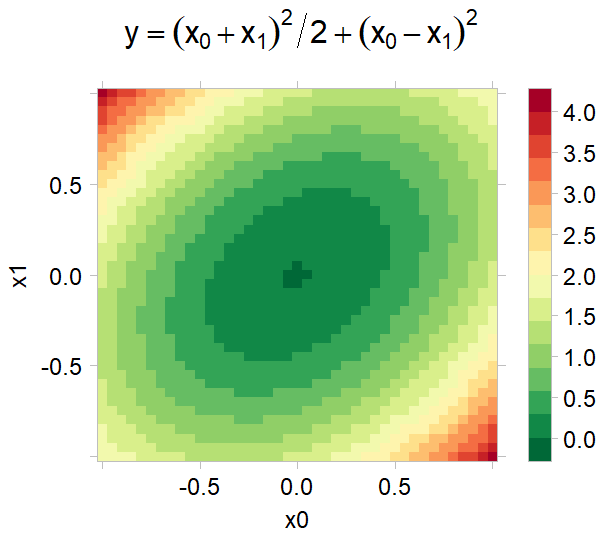
\includegraphics[width=80mm]{../fig/reg-true-levelplot}~
 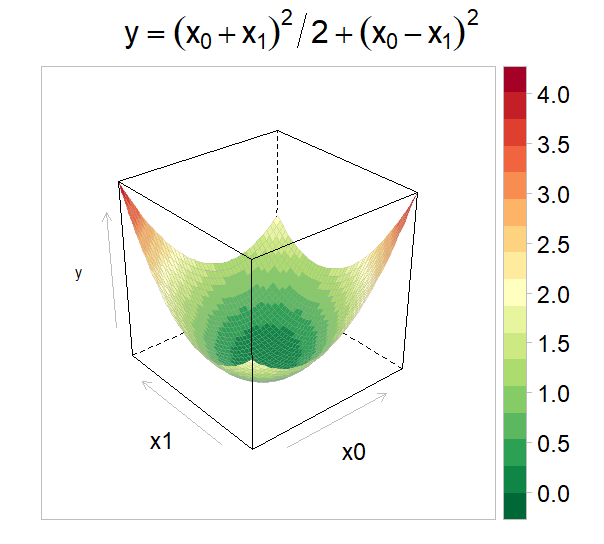
\includegraphics[width=80mm]{../fig/reg-true-wireframe}~
 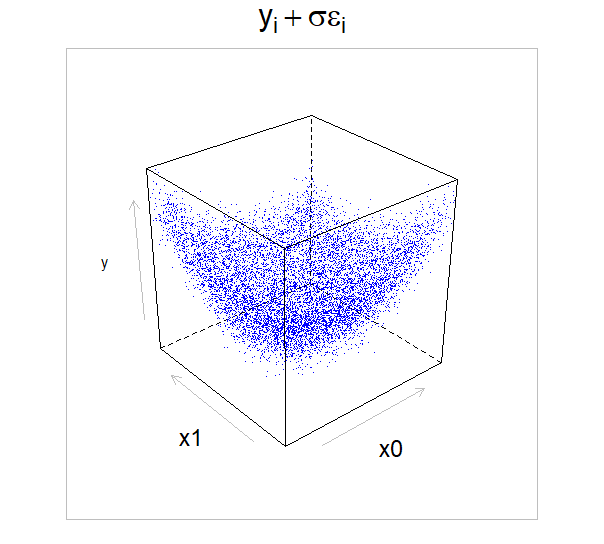
\includegraphics[width=80mm]{../fig/rpart-training-data}
\par\end{centering}

\protect\caption{\label{fig:synthetic-data}Synthetic data for regularization examples}
\end{figure*}



\subsection{\label{ite:Cross-validation}Cross validation (CART)}

CART \cite{breiman-friedman-olshen-stone-1984,hastie-tibshirani-friedman-2009}
is probably the most successful single regression tree method. CART
produces a binary tree which recursively partitions $\Xspace$ into
rectangular regions, each of which is fit by a constant value. The
model function $\f(\x_{i})$ finds which leaf/rectangular region of
the tree $\x_{i}$ is in, and returns the constant associated with
that leaf. 

CART has 2 phases: (1) a greedy tree growing phase common to most
tree-based methods and (2) a cross-validated pruning phase, which
is what makes CART special. 


\subsubsection{Greedy tree growth}

\begin{figure*}
\noindent \begin{centering}
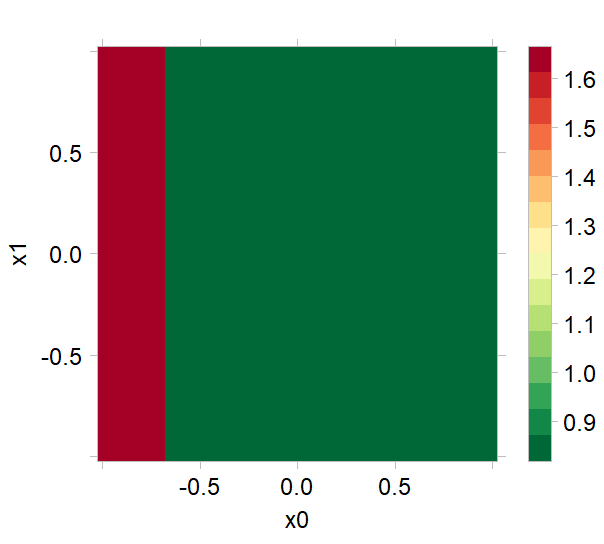
\includegraphics[width=80mm]{../fig/rpart-1-split-levelplot}~
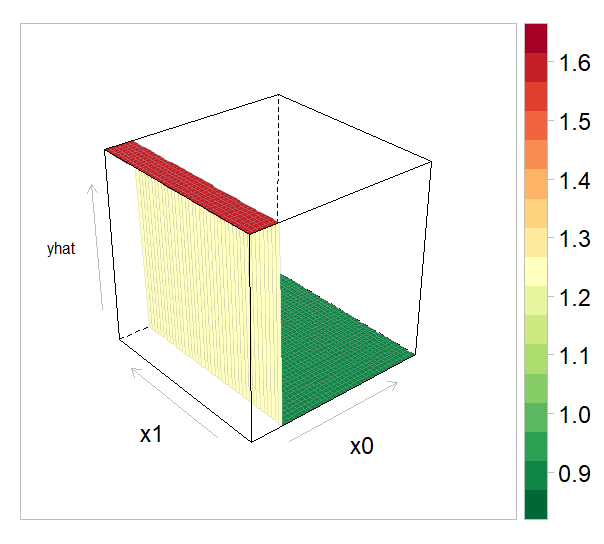
\includegraphics[width=80mm]{../fig/rpart-1-split-wireframe}~
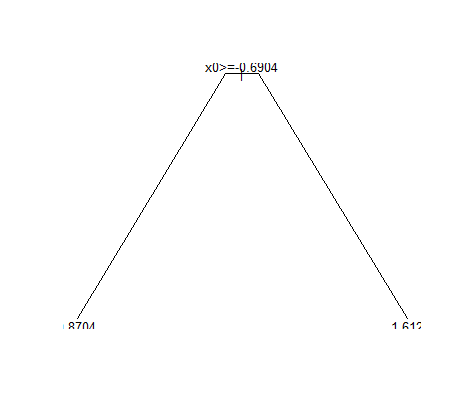
\includegraphics[width=80mm]{../fig/rpart-1-split-tree}
\par\end{centering}

\protect\caption{\label{fig:one-split}First split}
\end{figure*}


The growing phase is a optimizes the tree to minimize a cost function
over a training data set. In the case of least squares regression:
$\cost\left(\f,\mathcal{S}\right)=\sum_{(\x_{i},\y_{i})\in\mathcal{S}}(\y_{i}-\f(\x_{i}))^{2}$,
where $\mathcal{S}=\left\{ (\x_{i},\y_{i})\right\} $is a set of training
pairs.

To begin, we take the whole training set $\mathcal{S}$, and consider
every possible way of partitioning $\mathcal{S}=\mathcal{S}_{0}+\mathcal{S}_{1}$
using any one of the attributes in $\Xspace.$ For numerical attributes,
this means searching over predicates like $x_{1}\geq0.74$. For categorical
attributes, we need to consider all possible subsets of the categories.
For any contemplated split, we compute $\f_{\mathcal{S}_{k}}()=\argmin_{\f}\cost(\f,\mathcal{S}_{k})$
for each of the 2 possible subsets. In the most common case, we only
consider functions that are constant over the subset of the domain,
and $\f_{\mathcal{S}_{k}}()=\mean\left\{ \y_{i}:(\x_{i},\y_{i})\in\mathcal{S}_{k}\right\} $We
take the split that minimizes $\cost(\f_{\mathcal{S}_{0}},\mathcal{S}_{0})\,+\,\cost(\f_{\mathcal{S}_{1}},\mathcal{S}_{1})$.
The result of this process with our synthetic data is shown in figure
\ref{fig:one-split}. Then we repeat on the 2 leaves generated by
the first split, whose result is shown in figure \ref{fig:3-spits}.

\begin{figure*}
\noindent \begin{centering}
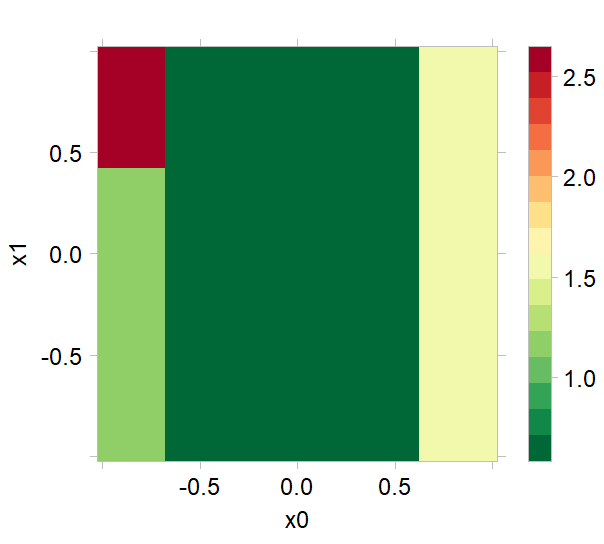
\includegraphics[width=80mm]{../fig/rpart-3-split-levelplot}~
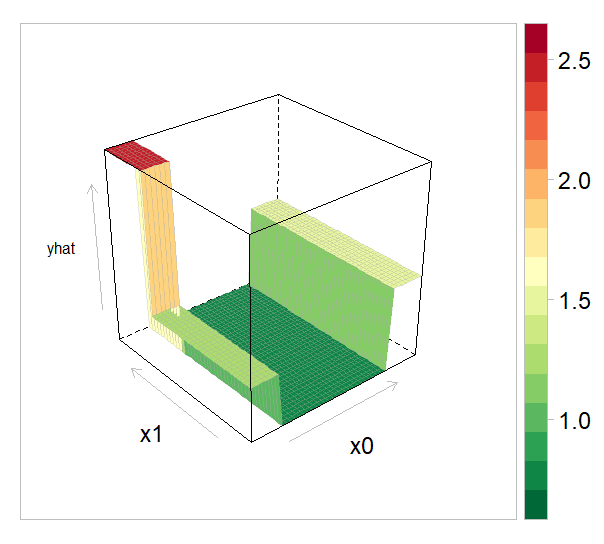
\includegraphics[width=80mm]{../fig/rpart-3-split-wireframe}~
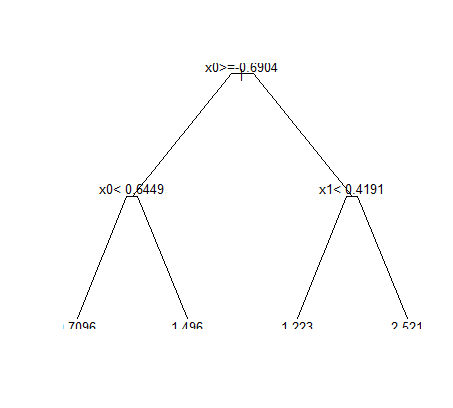
\includegraphics[width=80mm]{../fig/rpart-3-split-tree}
\par\end{centering}

\protect\caption{\label{fig:3-spits}First 3 splits}
\end{figure*}


This process continues until we run out of data, where 'run out of
data' means the training examples in a given node are either too few
or too similar to split meaningfully. The result is shown in figure
\ref{fig:unpruned-tree}

\begin{figure*}
\noindent \begin{centering}
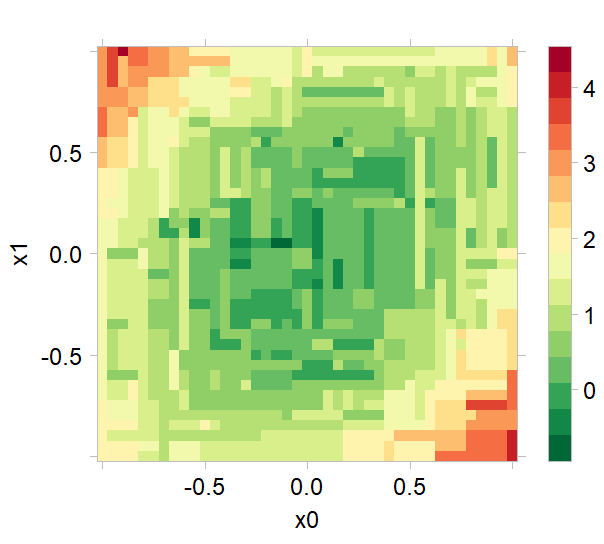
\includegraphics[width=80mm]{../fig/rpart-unpruned-levelplot}~
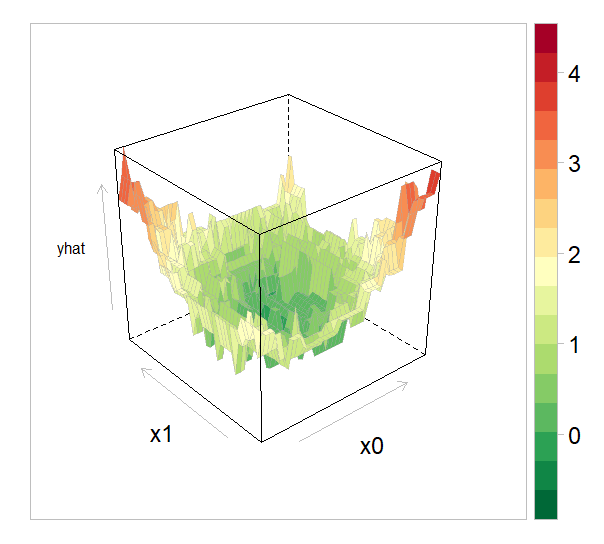
\includegraphics[width=80mm]{../fig/rpart-unpruned-wireframe}~
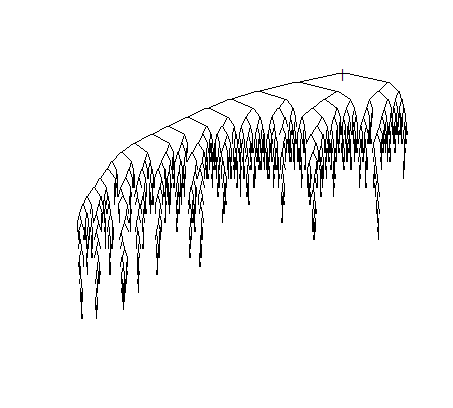
\includegraphics[width=80mm]{../fig/rpart-unpruned-tree}
\par\end{centering}

\protect\caption{\label{fig:unpruned-tree}Unpruned tree}
\end{figure*}


The fit is visually noisy and more important, could be shown by experiments
to give poor predictions of $\y$ given $\x$.


\subsubsection{Cross-validated pruning}

The key idea in CART was to use cross-validated pruning to fix the
tree shown in figure \ref{fig:unpruned-tree}.

Cross-validated pruning is a special case of cross-validated regularization,
which can be applied to almost any predictive modeling method. The
basic idea is to split the training data into 2 parts, training $\Tset_{0}$
and test $\Tset_{1}.$ We add a complexity term $\cmplxty()$ to the
cost that biases us towards simpler models. In the case of tree-based
models, this may be as simple as the number of nodes in the tree.
We have a parameter $\lambda$ that determines the relative tradeoff
between goodness of fit and complexity. 

For any given $\lambda$ we can find the optimal model by purely greedy
optimization:

\begin{equation}
\f_{\lambda}=\argmin_{\f\in\Fspace}\left[\lambda\cmplxty(\f)\;+\;\sum_{(\x_{i},\y_{i})\in\Tset_{0}}d\left(\y_{i},\f(\x_{i})\right)\right]
\end{equation}


We then need to choose an optimal value for $\lambda$. We do this
by optimizing the unregularized goodness of fit over the test data:

\begin{equation}
\f=\argmin_{\f_{\lambda}}\left[\sum_{(\x_{i},\y_{i})\in\Tset_{1}}d\left(\f_{\lambda}(\y_{i},\x_{i})\right)\right]
\end{equation}


It's usually not feasible to actually find the optimal $\f_{\lambda}$
for all values of $\lambda.$ Practical tree-based algorithms, like
CART first find the naive, unregularized $\f_{\lambda=0}$ and then
construct a heuristic sequence of smaller trees corresponding to increasing
values of $\lambda$. In CART this is done by collapsing splits from
the bottom up, always collapsing the split with the least improvement
$\cost(\f_{\mathcal{S}},\mathcal{S})\,-\,\cost(\f_{\mathcal{S}_{0}},\mathcal{S}_{0})\,-\,\cost(\f_{\mathcal{S}_{1}},\mathcal{S}_{1})$.
The cost as a function of tree size for our example is shown in figure
\ref{fig:Cross-validated-accuracy-vs}.

\begin{figure*}
\noindent \begin{centering}
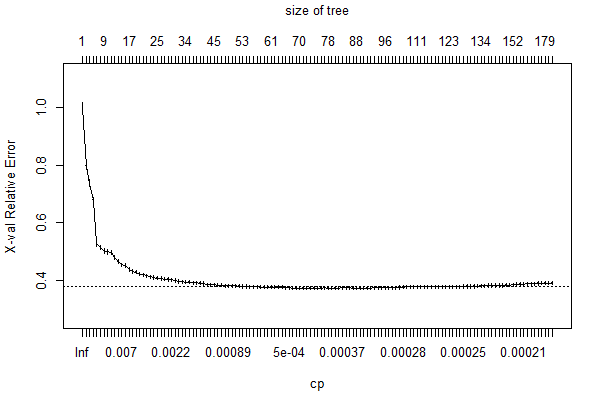
\includegraphics[width=12cm]{../fig/rpart-unpruned-plotcp}
\par\end{centering}

\protect\caption{\label{fig:Cross-validated-accuracy-vs}Cross-validated accuracy vs
tree size}
\end{figure*}


CART then picks the smallest tree such that no larger tree shows a
significant improvement. The result is in figure \ref{fig:pruned-tree}.
The resulting function is a pretty coarse approximation to the underlying
parabola.

\begin{figure*}
\noindent \begin{centering}
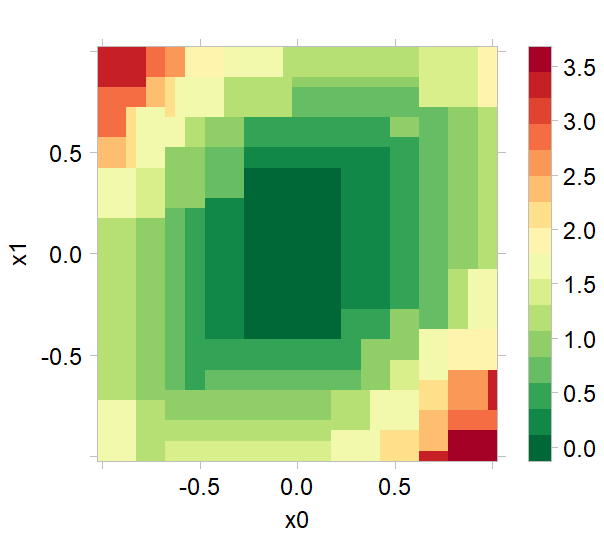
\includegraphics[width=80mm]{../fig/rpart-pruned-levelplot}~
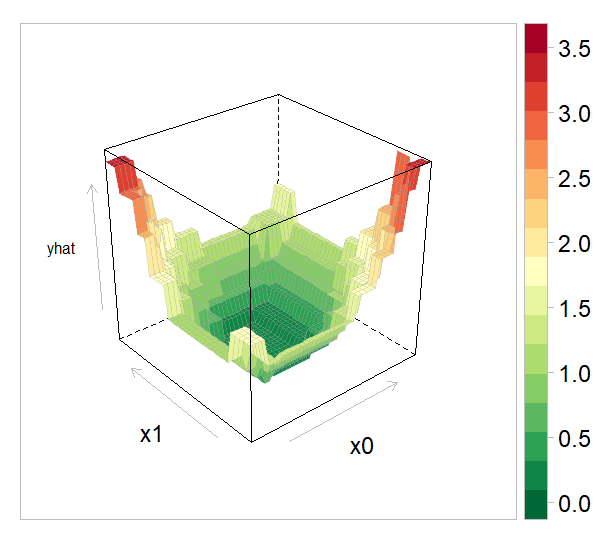
\includegraphics[width=80mm]{../fig/rpart-pruned-wireframe}~
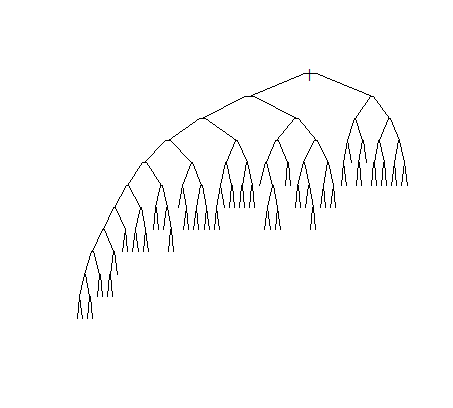
\includegraphics[width=80mm]{../fig/rpart-pruned-tree}
\par\end{centering}

\protect\caption{\label{fig:pruned-tree}Pruned tree}
\end{figure*}

\subsection{Bagging (Random Forests)}

Empirically, CART regression models perform about as well as any alternative.
However, there are at least 2 issues with single tree methods that
led to the development of forest-based methods. One, the crudeness
of the step function approximation shown in figure \ref{fig:pruned-tree}
is unsatisfying, especially in contexts where one believes $\y$ is
a smooth function of $\x$. Perhaps more important, single tree models
are inherently unstable, in the sense that small changes in the training
data result in completely different partitioning trees. The resulting
step function changes much less, but small regions close to the boundaries
of the steps can experience large jumps.

To prevent this, forest-based methods compute many trees$\f_{i}$
and then take as the final model $\f=\mathrm{{average}\left\{ \f_{i}\right\} }$,
where the average operation is defined appropriately for the problem.
For traditional regression problems, we just take the mean of the
predictions of the trees in the forest. In the transit time problem,
each $\f_{i}$ might be a histogram, or, equivalently, a cdf, and
the average would be just the numerical mean of the cdf or histogram
functions. 

Random forest is a particularly simple forest-based method, combining
bagging with randomly de-optimized tree growth.

The basic idea of bagging\label{ite:Bagging-(Random-Forests)} is
to simulate what we might see in future data by collecting $n$ independent
bootstrap (with-replacement) samples $\Tset_{_{i}}$ from the complete
training data $\Trainset$. We fit a model $\f_{i}$ via some base
learner to each bootstrap sample set $\Tset_{_{i}}$, and average
the results.

In practice, bagging alone is not very successful, unless it's coupled
with some further randomization or constraint that makes the individual
$\f_{i}$ less greedy. 

Random forests \cite{breiman-2001-machine-learning,hastie-tibshirani-friedman-2009}
uses the same greedy optimization as CART to grow its trees, except
that for each split it restricts the search to a random subset of
the attributes. Random forests are generally regarded as the most
successful method for regression and classification, but the reasons
for their success are not fully understood.

Figures \ref{fig:One-tree-random} thru \ref{fig:random-forest} illustrate
the process of creating a random forest on the same synthetic data.
Figure \ref{fig:Error-on-independent} shows how prediction accuracy
depends on the number of trees in the forest.

The final fit is much smoother than the CART model, but the increase
in overall accuracy over CART is relatively small. One reason people
tend to prefer random forests is that the error in random forest models
tends to be evenly distributed over the domain, whereas in CART models
it's more likely to be concentrated near the boundaries of the leaf
rectangles.

\begin{figure*}[t]
\noindent \begin{centering}
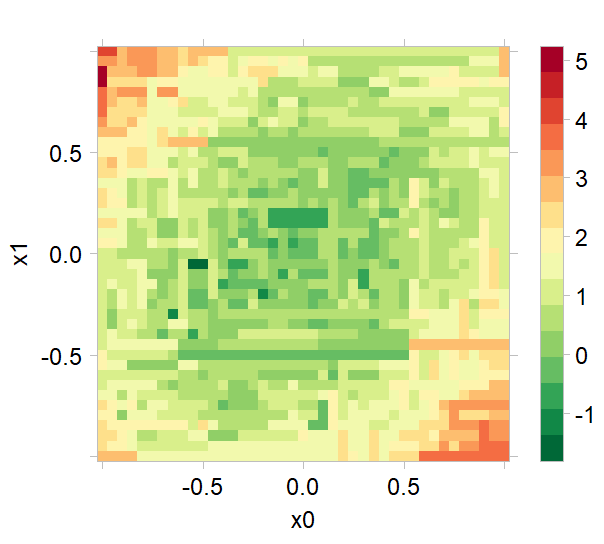
\includegraphics[width=80mm]{../fig/rf-1-tree-levelplot}~
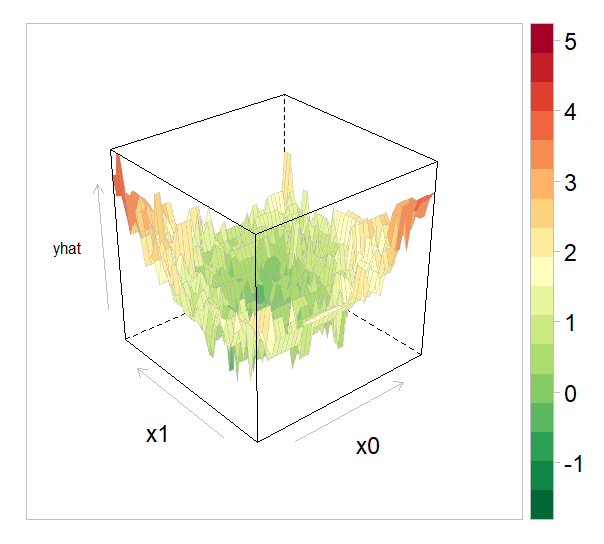
\includegraphics[width=80mm]{../fig/rf-1-tree-wireframe}
\par\end{centering}
\protect\caption{\label{fig:One-tree-random}One tree random forest}
\end{figure*}


\begin{figure*}
\noindent \begin{centering}
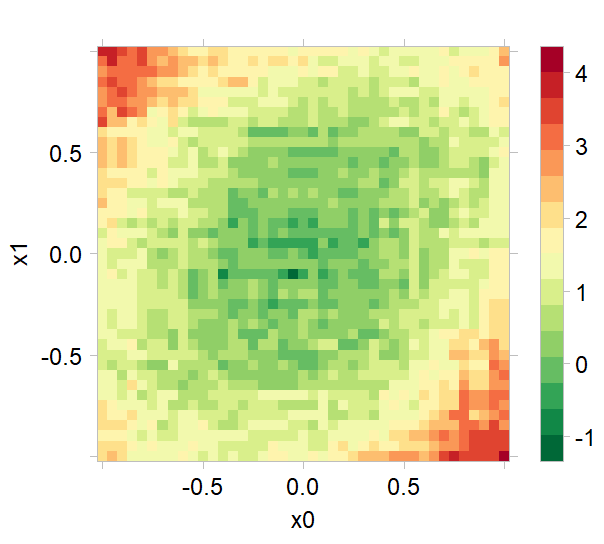
\includegraphics[width=80mm]{../fig/rf-4-tree-levelplot}~
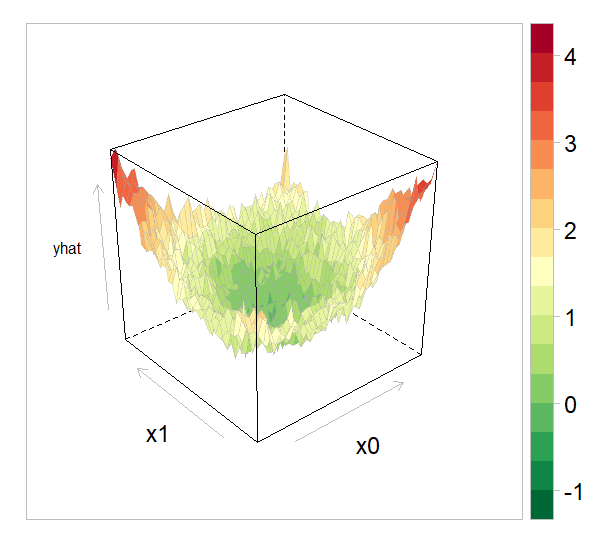
\includegraphics[width=80mm]{../fig/rf-4-tree-wireframe}
\par\end{centering}
\protect\caption{\label{fig:four-tree-random}Four tree random forest}
\end{figure*}


\begin{figure*}
\noindent \begin{centering}
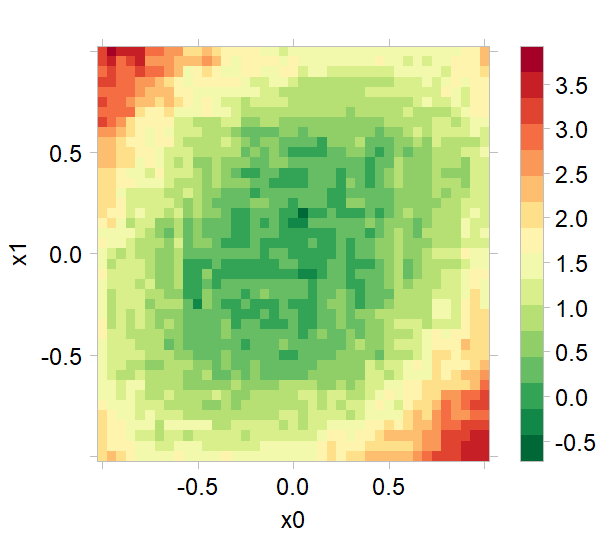
\includegraphics[width=80mm]{../fig/rf-1024-tree-levelplot}~
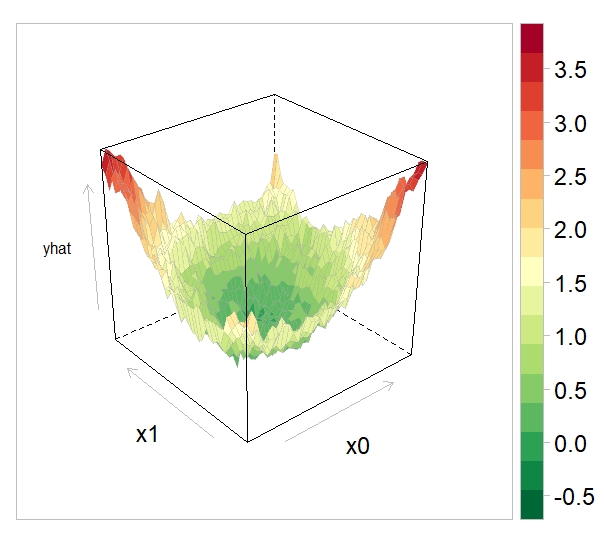
\includegraphics[width=80mm]{../fig/rf-1024-tree-wireframe}
\par\end{centering}

\protect\caption{\label{fig:random-forest}Complete random forest}
\end{figure*}
\begin{figure*}
\noindent \begin{centering}
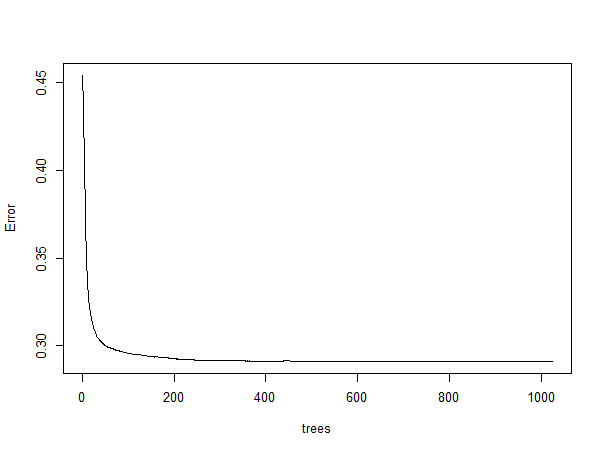
\includegraphics[width=12cm]{../fig/rf-1024-tree-forest}
\par\end{centering}

\protect\caption{
\label{fig:Error-on-independent}Error on test data by number of trees.}
\end{figure*}


\newpage{}

\section{\label{sec:Implementing-random-forest}Implementing random forest
regression}

The goal of this section is to walk you thru an implementation of
random forest regression.

If you are comfortable with Clojure and generally familliar with decision
trees, you should be able to get a working version in a day or 2.
At this point, we are looking for simplicity and generality, rather
than speed. The resulting code should be not much longer than the
high level description in Algorithm \ref{thm:Random-Forests-for}
(essentially Algorithm 15.1 from \cite{hastie-tibshirani-friedman-2009}),
except for steps 2b (section \ref{sub:Split-optimization}) and 2c
(section \ref{sub:Decision-trees}), where the details have obviously
been omitted.
\begin{algorithm}
\label{thm:Random-Forests-for}Random Forests for Regression or Classification. 

Training data $\mathcal{T}=\left\{ (\mathbf{x}_{i},y_{i});\,i=1\ldots N_{\textrm{records}}\right\} $.

For $k$ = $1$ to $N_{\textrm{trees}}$: 
\begin{enumerate}
\item Draw a bootstrap sample $\mathcal{T}_{k}$ from the training data. 
\item Grow a random-forest tree $f_{k}$ from each bootstrap sample $\mathcal{T}_{k}$,
by recursively repeating the following steps for each terminal node
of the tree, until the minimum node size $N_{\min}$ is reached. 

\begin{enumerate}
\item Select $m$ attributes at random from the total $p$ attributes. 
\item Pick the best attribute/split-point among the $m$.
\item Split the node into two daughter nodes. 
\end{enumerate}
\end{enumerate}
Return the ensemble $\mathcal{F}=\left\{ f_{k}\right\} $ . 

Prediction at $\mathbf{x}$: 
\begin{enumerate}
\item Regression: Use ensemble mean 
$f_{\mathcal{F}}(\mathbf{x})=\frac{1}{\#\mathcal{F}}\sum_{k}f_{k}(\mathbf{x})$. 
\item Classification: Use ensemble mode 
$f_{\mathcal{F}}(\mathbf{x})=\argmax_{c}\left(\#\left\{ f_{k}(\mathbf{x})=c\right\} \right)$
\item Probability: Use ensemble vote fraction.
\end{enumerate}
\end{algorithm}

We are going to do this backwards/top-down, so we start with general
ensemble (map-reduce) models:


\subsection{Ensemble models}

Random forests are a special case of additive models: 
$f(\mathbf{x})=\sum_{k}f_{k}(\mathbf{x})$.
In the random forest case, the terms, $f_{k}$, happen to all be regression
trees, but there's no reason to impose that restriction on our additive
model implementation. A simple additive model implementation in Clojure
is just a few lines of code (Listing \ref{lis:sum-model}), but it
demonstrates fundamental features of Lisp: higher order functions,
lexical scoping, and closures.

\begin{lstlisting}[caption={Sum additive model},label={lis:sum-model},language=clojure,tabsize=2]
(defn sum-model [terms] 
  (let [f (apply juxt terms)]
    (fn [x] (reduce + (f x)))))
\end{lstlisting}

\texttt{sum-model} takes a sequence of term functions as its single
argument, and returns a new function that computes the sum of the
values of the terms applied to the same argument \texttt{x}. Functions
that create new functions from old are sometimes referred to as 'higher
order functions', though there is really nothing special about them. 

We first use the Clojure (higher order) function \texttt{juxt}, which
creates a function that returns the sequence of the values of the
functions that are its arguments. \texttt{juxt} is defined for calls
like \texttt{((juxt~f~g)~x) -> {[}(f~x)~(g~x){]}}, so we use
\texttt{apply} to use it on a sequence of functions. 

The value of the \texttt{juxt} call is bound to the symbol \texttt{f},
which is referenced in the anonymous function, defined by the \texttt{(fn~{[}x{]}~(reduce...))}
expression, which use reduce to compute the sum of the sequence of
values returned by \texttt{f}.

The anonymous function returned by \texttt{sum-model} is an example
of what's often called a 'closure', because it uses the value of a
binding visible in the lexical scope at function definition time,
even though, in some sense that binding disappears once the call to
\texttt{sum-model} returns.

\subsection{\label{sub:Bagging}Bagging}

One way to generate an additive model is by \emph{bagging} (\textbf{b}ootstrap
\textbf{ag}gregation). We generate an ensemble of slightly different
models by applying a base learner to bootstrap samples from the training
data, and then combine predictions from the individual models to get
the ensemble prediction.

Note that bagging doesn't require the base learner to return decision
trees, or regression models, etc. Our implementation shouldn't make
those assumptions either.

\emph{Bootstrap sample} just means sampling training records with
replacement, generating a new data set that has on average something
like 2/3s the distinct records from the original data set, with exponentially
decaying numbers of records that are replicated once, twice, three
times, etc. 

Listing \ref{lis:bootstrapping} shows code from the supporting
\texttt{stat.random} library:

\begin{minipage}[t]{1\columnwidth}%
\begin{lstlisting}[caption={Bootstrapping},label={lis:bootstrapping},language=clojure,tabsize=2]
(defn sample-with-replacement [data prng]
  (let [n (count data)]
    (repeatedly n (fn [] (nth data (.nextInt ^Random prng n))))))
\end{lstlisting}
%
\end{minipage}
\begin{description}
\item [{Note~1:}] \texttt{sample-with-replacement} returns a lazy sequence,
meaning the samples from \texttt{data} won't be drawn until somebody
looks at them. This has a perhaps not-so-obvious implication: Until
it is fully realized, the lazy sequence will retain a reference to
\texttt{data}, so it won't be available for garbage collection.
\item [{Note~2:}] \texttt{\textasciicircum{}Random} is Clojure syntax
for a local type hint. \texttt{(.nextInt~\textasciicircum{}Random~prng~n)}
is equivalent to the Java expression \texttt{((Random)~prng).nextInt(n)}. 
\end{description}
Here's code for bagging a sequence of learners:

\begin{lstlisting}[caption={Bagging},label={lis:bagging},language=clojure,tabsize=2]
(defn bagging [data prng learners combine]
  (let [bags (repeatedly 
               (fn [] (sample-with-replacement data prng)))
        terms (map (fn [l b] (l b)) learners bags)]
    (combine terms))) 
\end{lstlisting}

\begin{description}
\item [{\texttt{data}:}] A collection of training pairs.
\item [{\texttt{prng}:}] A pseudo-random number generator.
\item [{\texttt{learners}:}] A (lazy) sequence of learners, each a function
that takes collection of training pairs and returns a (predictive
model) function.
\item [{\texttt{combine}:}] A function (like \texttt{mean-model} from exercise
\ref{Ex:mean-model}) that combines a (lazy) sequence of model functions
into a single model.
\item [{\texttt{bags}:}] A lazy infinite sequence of bootstrap samples
from \texttt{data}.
\item [{\texttt{terms}:}] A lazy sequence of model functions (eg trees)
produced by applying each learner to the corresponding bag. This will
be an infinite sequence if \texttt{learners} is infinite, in which
case it would by up to \texttt{combine} to determine how many terms
to actually compute. \end{description}

\subsection{\label{sub:Decision-trees}Decision trees}

A general binary decision tree consists of 
\begin{itemize}
\item internal \emph{split} nodes, each containing a predicate that determines
whether a record goes to the left or right child of that node.
\item terminal \emph{leaf} nodes, each containing a leaf model function
whose value is the tree's prediction for any record that ends up in
that node. 
\end{itemize}

\subsubsection{clojure.zipper}

The implementation here uses the \texttt{clojure.zip} package for
growing trees. The problem it solves for us is the following: 

To be able to safely use concurrency in random forest learning and
prediction, we need to rigorously minimize the amount of mutable shared
state. In particular, we want our trees, once grown, to be immutable.
But growth implies change. One approach is to have 2 representations
for trees, a mutable one to use while growing, which gets replicated
in an immutable representation when growing is done. Besides more
than doubling the complexity the tree representation, this approach
is problematic because tree growth itself is one of the places we'd
like to be free to use concurrency. 

\texttt{clojure.zip} manages traversing, and most important for us,
'editing' generic immutable tree-like data structures. clojure.zip
has a purely functional interface:\\
\texttt{ (clojure.zip/zipper~fertile?~get-children~get-node~root)
}\\
which returns a edit location that can be moved around a tree with
\texttt{(down~loc)}, \texttt{(left~loc)}, \texttt{(next~loc)},
etc., and that can be used to 'modify' an immutable tree with \texttt{(replace~loc~node)},
\texttt{(insert-left~loc~node)}, etc.

In the call to \texttt{zipper}, \texttt{root} is an instance of our
tree node representation, the root of the initial tree.

The first 3 arguments to \texttt{zipper} are functions with the signatures
below, where \texttt{node} is an instance of our tree node representation,
and \texttt{children} is a \texttt{seq} of instances of our node representation. 
\begin{description}
\item [{\texttt{(fertile?~node)}}] Answers the question: 'Can this node
have children?' (as opposed to 'Does this node have
children?').\footnote{Referred to as '\texttt{branch?}' in the Clojure 
documentation, one of many examples of the Clojure authors' difficulty
with the  English language.}
\item [{\texttt{(get-children~node)}}] What it says.
\item [{\texttt{(get-node~node~children)}}] Return a node that has \texttt{children}
as its children, possibly using \texttt{node} to initialize the returned
node.\footnote{Referred to as '\texttt{make-node}' in the Clojure documentation,
which even more misleading than '\texttt{branch?}'. Most tree representations
in Clojure will be immutable. If so, then there's no reason to construct
a new node if we already have one that has the specified children,
and that would most likely be true of \texttt{node} itself.} 
\end{description}

\subsubsection{defrecord}

The tree implementation described here uses several cooperating \texttt{defrecord}s
to implement the zipper API. This is only one of many reasonable choices
(and, given the hacky/afterthought/work-in-progress feel of \texttt{defrecord},
\texttt{defprotocol}, etc., perhaps not the best one).

Advantages include:
\begin{itemize}
\item compact syntax for dynamic creation of Java classes. 
\item all fields final, so instances are immutable if all field values are. 
\item general purpose Clojure functions are defined for each method, so
that methods can be passed to \texttt{map}, \texttt{comp}, \texttt{juxt},
etc. (which isn't true for methods defined in ordinary Java
classes)\footnote{This,  of course, raises the question: Why not do
this, as needed, for all Java classes?} .
\item the generated Java class automatically implements the Clojure key-value
map API:

\begin{itemize}
\item faster and more compact, especially if type hints are added to fields,
than using a general key-value map.
\item clone-able immutable prototypes via \texttt{(merge instance \{:field
value\})}
\end{itemize}
\end{itemize}
The disadvantages all reflect a number of mystifyingly bad design
choices:
\begin{itemize}
\item record definitions are not first class:

\begin{itemize}
\item no anonymous record definitions.
\item record definitions 'public', with global dynamic scope.
\item record definition can only be done thru macro call, no corresponding
function call.
\item serialization broken as of Clojure 1.3.
\item no meta-object protocol, inspection requires cumbersome Java reflection,
and so on.
\end{itemize}
\item only methods specified by a pre-existing Java interface can be defined,
imposing exactly the kind of type constraint you don't want in a dynamic
language.
\item fields are all public, making encapsulation impossible. 
\item field access via keywords rather than method/function needlessly complicates
field <-> method refactoring.
\item default constructor doesn't do any input validation, no mechanism
to add validation.
\item no inheritance, no code reuse.\end{itemize}

\subsubsection{Static trees and prediction}

We create the required Java interface with \texttt{defprotocol}:

\begin{minipage}[t]{1\columnwidth}%
\begin{lstlisting}[caption={Tree node protocol},label={lis:node-protocol},language=clojure,tabsize=2]
(defprotocol Node
  (fertile? [node])
  (get-children [node])
  (get-node [node children])) 
\end{lstlisting}
%
\end{minipage}

This just specifies the 3 functions/methods we will pass to the zipper
API. 

We need representations for terminal leaf nodes and internal split
nodes:

\begin{minipage}[t]{1\columnwidth}%
\begin{lstlisting}[caption={Leaf nodes},label={lis:leaf-defrecord},language=clojure,tabsize=2]
(defrecord Leaf [model]
  Node
  (fertile? [leaf] false)
  (get-children [leaf] nil)
  (get-node [leaf children] leaf)) 
\end{lstlisting}
%
\end{minipage}

A \texttt{Leaf} has one field, whose value is the model function to
be applied to any case that ends up in that leaf. Because leaves are
terminal, they aren't fertile (can't have children). We are assuming
that the model is immutable, so it's safe to return the leaf itself
from the \texttt{get-node} method. 

\begin{minipage}[t]{1\columnwidth}%
\begin{lstlisting}[caption={Split nodes},label={lis:split-defrecord},language=clojure,tabsize=2]
(defrecord Split [predicate true-child false-child]
  Node
  (fertile? [branch] true)
  (get-children [branch] (seq [true-child false-child]))
  (get-node [branch children] 
    (Split. predicate (first children) (second children)))) 
\end{lstlisting}
%
\end{minipage}

A Split has 3 fields, whose values are the \texttt{predicate} function
determining which cases go to which child, and the children corresponding
to whether the predicate returns \texttt{true} or \texttt{false}. 

\begin{minipage}[t]{1\columnwidth}%
\begin{lstlisting}[caption={Generic prediction},label={lis:predict},language=clojure,tabsize=2]
(defn predict [node x]
  (if (instance? Split node)
    (if ((:predicate node) x)
      (recur (:true-child node) x)
      (recur (:false-child node) x))
	((:model node) x)))

(defn tree-model [root] (fn [x] (predict root x))) 
\end{lstlisting}
%
\end{minipage}

Prediction is done by the simple recursive \texttt{predict} function
in listing \ref{lis:predict}\footnote{One of the quirks of Clojure is that it requires the programmer to
identify opportunities for tail-call optimization and exploit manually
them by calling \texttt{recur} in place of the function name, even
though \texttt{defn/fn} could fairly easily do the equivalent for
you.}. To get a model function we can, for example, use as a term in an
additive mode, we need only construct a one-line closure as in \texttt{tree-model}.

The key thing to note is that so far, this tree implementation doesn't
depend on what kind of tree model it is, regression, classification,
survival, etc. It also doesn't depend on the nature of \texttt{x},
which might be a tuple of primitive fields (as in most implementations
of decision trees), but could easily be a time series, a bag of terms,
a polygon in a spatial mesh, or anything else.

\subsubsection{Tree growing}

To support learning trees from training data, I add a 3rd implementation
of \texttt{Node}, called \texttt{Bud}. The job of a \texttt{Bud} is
to carry shrinking subsets of training pairs down the tree, and 'sprout',
creating either a \texttt{Leaf} node, or a \texttt{Split} node with
2 new \texttt{Bud}s as children. 

\begin{minipage}[t]{1\columnwidth}%
\begin{lstlisting}[caption={Buds},label={lis:bud-defrecord},language=clojure,tabsize=2]
(defrecord Bud [leaf-learner split-learner pairs]
  Node
  (fertile? [bud] false)
  (get-children [bud] nil)
  (get-node [bud children] bud)) 
\end{lstlisting}
%
\end{minipage}

The fields:
\begin{description}
\item [{\texttt{leaf-learner}:}] A function that returns a model given
a set of training pairs. For L2 regression, this would be something
like \texttt{(fn~{[}pairs{]}~(constantly~(mean~y~pairs))) }where
\texttt{(mean~y~pairs)} is the mean of the \texttt{y} attribute
in pairs, and \texttt{(constantly~z)} returns a constant function,
that is \texttt{((constantly~z)~x)} is \texttt{z} regardless of
\texttt{x}.
\item [{\texttt{split-learner}:}] A function that returns a split predicate
function given a set of training pairs. More detail in section \ref{sub:Split-optimization}.
\item [{\texttt{pairs}:}] A collection of \texttt{RegressionPairs}.
\end{description}
Functions that operate on \texttt{Bud}s:

\begin{minipage}[t]{1\columnwidth}%
\begin{lstlisting}[caption={(sprout bud)},label={lis:sprout},language=clojure,tabsize=2]
(defn sprout [bud]
  (let [predicate ((:split-learner bud) (:pairs bud))]
    (if predicate
      (split bud predicate)
      (leaf bud))))
\end{lstlisting}
%
\end{minipage}
\begin{description}
\item [{\texttt{sprout}}] applies the bud's split learner to its pairs,
returning either a predicate function, or \texttt{false} if the learner
believes the pairs shouldn't be split any further. Then either divides
the training data between 2 new \texttt{Bud}s or ends the tree growth
by returning a \texttt{Leaf}.
\end{description}
\begin{minipage}[t]{1\columnwidth}%
\begin{lstlisting}[caption={(split bud)},label={lis:split},language=clojure,tabsize=2]
(defn split [bud predicate]
  (let [groups (group-by (comp predicate :x) (:pairs bud))]
     (Split. predicate
             (merge bud {:pairs (get groups true)})
             (merge bud {:pairs (get groups false)}))))
\end{lstlisting}
%
\end{minipage}
\begin{description}
\item [{\texttt{split}}] constructs an instance of \texttt{Split} from
the bud and the predicate. Note the use of \texttt{merge} to 'clone'
2 new buds, updating only the pairs field.
\end{description}
\begin{minipage}[t]{1\columnwidth}%
\begin{lstlisting}[caption={(leaf bud)},label={lis:leaf},language=clojure,tabsize=2]
(defn leaf [bud]
  (let [model ((:leaf-learner bud) (:pairs bud))]
    (Leaf. model)))
\end{lstlisting}
%
\end{minipage}
\begin{description}
\item [{\texttt{leaf}}] constructs an instance of \texttt{Leaf}, getting
the model function by applying the bud's leaf learner to its pairs.
\end{description}

\subsubsection{Managing tree learning with clojure.zip}

We create a zipper from a \texttt{Bud} with:

\begin{minipage}[t]{1\columnwidth}%
\begin{lstlisting}[caption={Create a zipper for growing a tree},label={lis:zipper},language=clojure,tabsize=2]
(defn zipper [root] 
  (z/zipper fertile? get-children get-node root)) 
\end{lstlisting}
%
\end{minipage}

This will create a \texttt{clojure.zip} edit location object that
will use our definitions of \texttt{fertile?}, \texttt{get-children},
and \texttt{get-node} to navigate and edit the tree starting from
the supplied \texttt{root} bud\footnote{'\texttt{z/}' is short for '\texttt{clojure.zip/}', and assumes we
have done something like \texttt{(:require~{[}clojure.zip~:as~z{]})}
in defining our namespace.}. 

These are functions that use \texttt{clojure.zip} to walk over the
current, terminal buds, sprouting into leaves or splits with new buds,
where appropriate.

\begin{minipage}[t]{1\columnwidth}%
\begin{lstlisting}[caption={Growing a tree using a zipper},label={lis:grow-loc},language=clojure,tabsize=2]
(defn grow-loc [loc]
  (cond (z/end? loc) (z/root loc)
        (z/branch? loc) (recur (z/next loc))
        :else (recur (z/next (sprout-loc loc))))) 
\end{lstlisting}
%
\end{minipage}

Notes:
\begin{description}
\item [{\texttt{grow-loc}}] a recursive function that walks the edit location
\texttt{loc} depth first over the growing tree, finding buds to sprout.
\item [{\texttt{z/end?}}] true if we've reached the end of a depth first
traversal of the tree --- the \texttt{loc} doesn't point to a node,
but to a marker for end-of-iteration.
\item [{\texttt{z/root}}] returns the node at the root of the tree (not
an edit location pointing to the root).
\item [{\texttt{z/branch?}}] true if the node pointed to by \texttt{loc}
can have children, ie, is a \texttt{Split}. 
\item [{\texttt{z/next}}] returns an edit location pointing to the next
node in a depth first traversal of the tree.
\end{description}
\begin{minipage}[t]{1\columnwidth}%
\begin{lstlisting}[caption={Sprouting a bud using a zipper},label={lis:grow-loc-1},language=clojure,tabsize=2]
(defn sprout-loc [loc]
   (let [bud (z/node loc)
         new-node (sprout bud)]
     (z/replace 
       loc 
       (z/make-node loc new-node (get-children new-node)))))
 
\end{lstlisting}
%
\end{minipage}
\begin{description}
\item [{\texttt{sprout-loc}}] the \texttt{loc} must point to a \texttt{Bud}.
We then edit the tree, replacing the bud with the new \texttt{Split}
or \texttt{Leaf} returned from \texttt{sprout}.
\item [{\texttt{z/node}}] returns the \texttt{Node} pointed to by an edit
location \texttt{loc}.
\end{description}

\subsubsection{External interface for learning tree models}
\begin{minipage}[t]{1\columnwidth}%
\begin{lstlisting}[caption={Tree learner},label={lis:tree-learner},language=clojure,tabsize=2]
(defn learn [leaf-learner split-learner pairs]
  (let [root-loc (zipper (Bud. leaf-learner split-learner pairs))
        tree (grow-loc root-loc)
    (tree-model tree))) 
\end{lstlisting}
%
\end{minipage}

Note the use of \texttt{tree-model} from listing \ref{lis:predict},
to convert \texttt{tree} to a function.

\subsection{\label{sub:Split-optimization}Greedy split optimization}

At this point, we've implemented the major conceptual content of random
forests, in about 70 fairly short lines of Clojure. None of the code
so far depends on the fact that we are doing L2 numerical regression,
and could be used without change for classification, vector regression,
etc.

In this section I will describe split optimization, concretely: how
to implement the \texttt{split-learner} passed to \texttt{learn} in
listing \ref{lis:tree-learner}. This will require about as much code
as we've written so far. Though not strictly necessary, I will for
the first time introduce code that depends on the fact that L2 numerical
regression (for speed).


\subsubsection{Finding the best attribute}

The entry point for split optimization is \texttt{best-split}, which
returns a predicate function that defines the split.

\begin{minipage}[t]{1\columnwidth}%
\begin{lstlisting}[caption={Split optimization entry point},label={lis:best-split},language=clojure,tabsize=2]
(defn best-split [cost-factory acceptable? score pairs 
                  attributes]
  (let [split (partial attribute-split 
                       cost-factory acceptable? score pairs) 
        cost (comp :cost splitter)
        best-attribute (argmin cost attributes)
        s (split best-attribute)]
    (:predicate s))) 
\end{lstlisting}
%
\end{minipage}
\begin{description}
\item [{\texttt{cost-factory}:}] A function of no arguments that returns
an instance of \texttt{Accumulator} (see listing \ref{lis:accumulator}).
Each \texttt{Accumulator} is a cost function (such as the sum of squared
deviations from the mean) that can be efficiently updated/downdated
by adding/removing double precision numbers.
\item [{\texttt{acceptable?}:}] A predicate used to evaluate whether a
given split is allowed. For example, it may the constrain Leaf nodes
to have at least some minimum number of training records.
\item [{\texttt{score}:}] A double-valued function applied to groups of
training records, used to sort the groups corresponding to discrete
attributes. In L2 regression, the score function is just the mean
of the y-values in the group. In 2-class classification, it's the
fraction of training records in class 1.
\item [{\texttt{pairs}:}] Training data.
\item [{\texttt{attributes}:}] Attribute functions available for splitting.
\item [{\texttt{split}:}] Finds the best split for a given attribute. \texttt{partial}
constructs a function of one argument that calls \texttt{attribute-split}
(see listing \ref{lis:attribute-split}) with the first 4 arguments
set to the given values (this is often referred to as 'currying').
\item [{\texttt{cost}:}] A function the returns the cost of the best split
on a given attribute. \texttt{comp} returns a function that is the
composition of \texttt{:cost} and \texttt{splitter} --- this is assuming
that splitter returns a Map with the value of the best split it finds
in the \texttt{:cost} field.
\item [{\texttt{best-attribute}:}] The best attribute to split on. 
\item [{\texttt{s}:}] The best split on the best attribute, recomputed.
(The re-computation could be avoided at the cost of a slightly more
complicated version of \texttt{argmin}.) Assumed to be a Map with
a \texttt{:predicate} field containing the split predicate.\end{description}

\subsubsection{The best split on a given attribute}

\begin{minipage}[t]{1\columnwidth}%
\begin{lstlisting}[caption={Best split for a given attribute},label={lis:attribute-split},language=clojure,tabsize=2]
(defn attribute-split [cost-factory acceptable? score pairs 
                       attribute]
  (let [split (if (numerical? attribute) 
                numerical-split 
                categorical-split)] 
    (split cost-factory acceptable? score pairs attribute))) 
\end{lstlisting}
%
\end{minipage}

\texttt{attribute-split} just dispatches to the appropriate method
for numerical versus categorical attributes.

\subsubsection{Numerical splits}

To optimize a numerical split, we 
\begin{enumerate}
\item to handle ties correctly, group the training pairs on the value of
the x attribute.
\item sort the groups by increasing x.
\item replace the groups of pairs by groups of corresponding y values.
\item add all the y values to the right hand cost function.
\item move each group from right to left 
\item check whether the resulting split is acceptable.
\item update, if needed, the minimizing cost and x value.
\end{enumerate}
When done we return the minimum cost and the corresponding predicate
function in a map.

Every split is tested for acceptability, and, if no acceptable splits
are found, infinite cost and a nil predicate are returned.

\begin{minipage}[t]{1\columnwidth}%
\begin{lstlisting}[caption={Optimal split on a numerical attribute},label={lis:numerical-split},language=clojure,tabsize=2]
(defn numerical-split [cost-factory acceptable? score pairs
                       attribute]
  (let [groups (group-by :x pairs)
        groups (sort-by key groups)
        groups (map (fn [[x pairs]] [x (map :y pairs)]) groups)
        ^Accumulator cost0 (cost-factory)
        ^Accumulator cost1 (cost-factory)]
    (doseq [[_ ys] groups] (.addAll cost1 ys))
    (loop [gs groups
           xmin Double/NaN
           cmin Double/POSITIVE_INFINITY]
      (if-not (empty? gs)
        ; continue
        (let [[[x ys] & rgs] gs
              cost (double (+ (.deleteAll cost1 ys) 
                              (.addAll cost0 ys)))]
          (if (and (acceptable? cost0 cost1)
                   (< cost cmin)) 
            (recur rgs (double x) cost)
            (recur rgs xmin cmin)))
        ; done         
        (let [p (if-not (== Double/POSITIVE_INFINITY cmin)
                  (fn [x] (<= (attribute x) xmin)))]
          {:predicate p :cost cmin}))))) 
\end{lstlisting}
%
\end{minipage}

Note the use of a couple Clojure features:
\begin{description}
\item [{\emph{destructuring~bind:}}] Instead of just binding a name to
a value, Clojure also supports binding expressions containing names
to values. The value must have structure homolgous to the name expression,
and Clojure automatically takes apart the value, binding its pieces
to the corresponding pieces of the name expression. Concretely, \texttt{(let~{[}{[}{[}x
ys{]}~\&~rgs{]}~gs\ldots{}{]}\ldots{})} takes the first element
of the sequence \texttt{gs}, which must itself be a sequence whose
first element is a sequence, binds \texttt{x} to the first element
of the first element of \texttt{gs}, binds \texttt{ys} to the second
element of the first element of \texttt{gs}, and binds \texttt{rgs}
to the rest of \texttt{gs}.
\item [{\texttt{\emph{loop}}\emph{~special~form:}}] \texttt{loop} does
not actually do iterative looping as in C/Java's \texttt{for}, but
is really syntatic sugar equivalent to defining a recursive local
function, and then calling that function.\footnote{I'm not sure whether the \texttt{loop} syntatic sugar is helpful or
just confusing, but it would almost certainly be better to call it
something else. The \texttt{for} macro is definitely perverse, at
least its name.} 
\end{description}

\subsubsection{Categorical splits}

Many implementations of random forest regression either don't support
categorical attributes, or have arbitrary restrictions on the number
of categories (due mostly likely to the fact that they are derived
from the original implementation in Fortran, which is impoverished
in data structures compared to most modern languages).

The implementation here relies on the fact that, for numerical regression
and 2-class classification, we don't need to consider all possible
partitions of the categories into 2 subsets. Instead we can sort the
categories by the value of a score function, and only consider simple
numerical splits on the score. 

For regression, the score is the mean of the y values for all the
training cases with the given category.

For 2-class classification, it's the fraction of the training cases
with the given category whose y value is class 0.

\begin{minipage}[t]{1\columnwidth}%
\begin{lstlisting}[caption={Optimal split on a categorical attribute},label={lis:categorical-split},language=clojure,tabsize=2]
(defn categorical-split [cost-factory acceptable? score pairs 
                         attribute]
  (let [groups (group-by :x pairs)
        groups (sort-by (comp score val) groups)
        groups (map (fn [[x pairs]] [x (map :y pairs)]) groups)
        ^Accumulator cost0 (cost-factory)
        ^Accumulator cost1 (cost-factory)]
    (doseq [[x ys] groups] (.addAll cost1 ys))
    (loop [gs groups
           gmin groups
           cmin Double/POSITIVE_INFINITY]
      (if-not (empty? gs)
        ; continue
        (let [[[x ys] & rgs] gs
              cost (double (+ (.deleteAll cost1 ys) 
                              (.addAll cost0 ys)))]
          (if (and (acceptable? cost0 cost1)
                   (< cost cmin))
            (recur rgs rgs cost)
            (recur rgs gmin cmin)))
        ; done
        (let [p (if-not (== Double/POSITIVE_INFINITY cmin)
                  (let [cats (set (map first gmin))]
                    (fn [x] (contains? cats (attribute x)))))]
          {:predicate p :cost cmin} )))))
\end{lstlisting}
%
\end{minipage}

\subsubsection{Split constraints}

A simple split acceptability predicate is shown in

\begin{minipage}[t]{1\columnwidth}%
\begin{lstlisting}[caption={Minimum amount of training data in a leaf},label={lis:mincount-split},language=clojure,tabsize=2]
(defn mincount-split? [mincount cost0 cost1]
  (and (<= mincount (.count ^Accumulator cost0))
       (<= mincount (.count ^Accumulator cost1)))) 
\end{lstlisting}
%
\end{minipage}

This will ensure that every leaf has at least \texttt{mincount} training
cases.

\subsection{Cost functions for L2 numerical regression}

The cost function for L2 regression is the sum of squared deviations
from the mean: $L_{2}\left(\mathcal{T}\right)=\sum_{y\in\mathcal{T}}\,\left(y-\bar{y}\left(\mathcal{T}\right)\right)^{2}$,
where $\bar{y}\left(\mathcal{T}\right)=\frac{1}{\#\mathcal{T}}\sum_{y\in\mathcal{T}}\,y$.
Computing this accurately in an online fashion, allowing for the updating/downdating
needed for fast split optimization, requires some care. An implementation
that does this efficiently and accurately is provided in \texttt{stat.stats/MeanSSE}.

However, a little bit of algebra will let us use an even simpler alternative
to get the same splits. Any split partitions the training y-values
$\mathcal{T=}\left\{ y\right\} $ into left and right subsets: $\mathcal{T}=\mathcal{L}\uplus\mathcal{R}$.
The split cost is:

\begin{align*}
c\left(\mathcal{L},\mathcal{R}\right)= & L_{2}\left(\mathcal{L}\right)+L_{2}\left(\mathcal{R}\right)\\
= & \sum_{y\in\mathcal{L}}\,\left(y-\bar{y}\left(\mathcal{L}\right)\right)^{2}+\sum_{y\in\mathcal{R}}\,\left(y-\bar{y}\left(\mathcal{R}\right)\right)^{2}\\
= & \sum_{y\in\mathcal{L}}\left[y^{2}-2\bar{y}\left(\mathcal{L}\right)y+\bar{y}\left(\mathcal{L}\right)^{2}\right]+\sum_{y\in\mathcal{R}}\left[y^{2}-2\bar{y}\left(\mathcal{R}\right)y+\bar{y}\left(\mathcal{R}\right)^{2}\right]\\
= & \sum_{\mathcal{L}\uplus\mathcal{R}}y^{2}-\frac{\left(\sum_{\mathcal{L}}y\right)^{2}}{\#\mathcal{L}}-\frac{\left(\sum_{\mathcal{R}}y\right)^{2}}{\#\mathcal{R}}
\end{align*}


Since $\sum_{\mathcal{L}\uplus\mathcal{R}}y^{2}$ doesn't depend on
the split, minimizing $c\left(\mathcal{L},\mathcal{R}\right)$ is
equivalent to minimizing $-\left[\frac{\left(\sum_{\mathcal{L}}y\right)^{2}}{\#\mathcal{L}}+\frac{\left(\sum_{\mathcal{R}}y\right)^{2}}{\#\mathcal{R}}\right]$,
so we can use $\frac{-\left(\sum_{\mathcal{T}}y\right)^{2}}{\#\mathcal{T}}$
as our cost function in split optimization.. An implementation of
this cost is provided in \texttt{stat.stats/MSSN}.

\subsection{Random forest split optimization}

Breiman's original idea was to apply bagging to decision trees, to
get smoother predictions than those returned by the best single decision
tree models like CART\cite{breiman-friedman-olshen-stone-1984}. (See
appendix \ref{sec:Predictive-modeling-with} for examples.) However,
bagged CART forests had worse prediction accuracy than single CART
trees in most problems, not to mention being $\approx10^{2}$ times
more expensive to compute. Replacing CART with cheaper alternative
approaches to regularized greedy trees, like restricting the depth
or the number of leaves, reduced computational cost, but didn't help
accuracy.

The change that made (what was eventually named) random forests work
well enough to be useful, was to replace regularized greedy trees
with unregularized trees using randomized, not-quite-greedy split
optimization. 

Greedy split optimization considers all the attributes in the training
data, choosing to split on the attribute whose best split most reduces
the cost function. 

Random forest split optimization selects a (different) random subset
of the attributes at each node, and chooses the best split, restricted
to that random subset. 

If this seems somewhat mysterious to you, you are in good company.
The arbitrariness of this is further emphasized by the fact that it
introduces a tuning parameter, the size of the random subset of the
attributes, without any real guidance for choosing the value of that
parameter. Breiman and Cutler recommended $m=\left\lfloor \frac{p}{3}\right\rfloor $
for regression problems and $m=\left\lfloor p^{\frac{1}{2}}\right\rfloor $
for classification problems, based on experience with a small number
of small data sets. ($m$ is the subset size and $p$ is the total
number of attributes.) However, varying $m$ away from the recommended
values often greatly improves prediction accuracy (see for example
\cite{hastie-tibshirani-friedman-2009} figure 15.4).

\begin{minipage}[t]{1\columnwidth}%
\begin{lstlisting}[caption={Random forest split optimizer},label={lis:random-forest-splits},language=clojure,tabsize=2]
(defn random-forest-splitter [attributes cost-factory splittable? 
                              score m prng]
  (fn [pairs]
    (let [a (sample m attributes prng)]
      (best-split cost-factory splittable? score pairs a)))) 
\end{lstlisting}
%
\end{minipage}

\texttt{random-forest-splitter} returns a function that does random
forest split optimization. Every time it's called, it selects a new
subset of the original list of attributes, and then applies the greedy
\texttt{best-split} function to choose the best split from the attribute
subset.


\subsection{Generic random forests}

Here's a generic random forest implementation --- generic in the sense
that it will do either classification or regression, depending on
the choices of \texttt{leaf-learner}, \texttt{cost-factory}, \texttt{score},
and \texttt{combine}.

\begin{minipage}[t]{1\columnwidth}%
\begin{lstlisting}[caption={Generic random forests},label={lis:random-forests},language=clojure,tabsize=2]
(defn random-forest [pairs attributes leaf-learner cost-factory
                     splittable? score combine ntrees m]

 (let [bag-prng (mersenne-twister-generator)
       prngs (repeatedly mersenne-twister-generator)
       make-splitter
         (partial random-forest-splitter 
                  attributes cost-factory splittable? score m)
       splitters (map make-splitter prngs)
       learners (map (fn [s] (partial tree/learn leaf-learner s)) 
                      splitters)]

    (bagging pairs bag-prng (take ntrees learners) combine)))  
\end{lstlisting}
%
\end{minipage}
\begin{description}
\item [{\texttt{bag-prng}}] a pseudo-random number generator used for bootstrap
samples.
\item [{\texttt{prngs}}] a lazy infinite sequence of random number generators,
for randomized split optimization in each tree.
\item [{\texttt{make-splitter}}] a splitter factory that curries out the
first 4 arguments to \texttt{random-forest-splitter}.
\item [{\texttt{splitters}}] a lazy infinite sequence of random forest
splitters.
\item [{\texttt{learners}}] a lazy infinite sequence of random forest tree
learners.
\end{description}
I keep the random forest finite by only passing the first \texttt{ntrees}
learners to \texttt{bagging}.

\subsection{\label{sub:Random-forest-regression}Random forest regression}

\begin{minipage}[t]{1\columnwidth}%
\begin{lstlisting}[caption={Random forest regression},label={lis:random-forest-regression},language=clojure,tabsize=2]
(defn regression [pairs attributes ntrees mincount]

  (let [score (fn [d] (mean :y d))
        leaf-learner (fn [d] (constantly (score d)))
        splittable? (partial mincount-split? mincount)
        m (max 1 (int (/ (count attributes) 3)))]

    (random-forest data leaf-learner mssn splittable? score
                   mean-model ntrees m)))
\end{lstlisting}
%
\end{minipage}

\subsection{Examples}

\subsection{Boston Housing (2)}

The Boston Housing Data\footnote{A little known fact: this data was originally collected by my older
brother, while an undergraduate. He's since gone on to bigger and
better things \cite{BostonHousing}.}, though tiny (506x19) by contemporary standards, has been a standard
test set for regression since the 1970s. Code that parses a tab-separated
file containing the data into appropriate regression training pairs,
using the tsv library described in section \ref{sub:util.tsv}, is
in listing \ref{lis:Reading-the-Boston}.

\begin{minipage}[t]{1\columnwidth}%
\begin{lstlisting}[caption={Boston housing record class},label={lis:Reading-the-Boston},language=clojure,tabsize=2]
(defrecord Record
   [^double lon ^double lat ^double crim ^double zn 
    ^double indus ^double nox ^double rm ^double age 
    ^double dis ^double rad ^double tax ^double ptratio
    ^double b ^double lstat ^boolean chas]) 

\end{lstlisting}
%
\end{minipage}

\begin{minipage}[t]{1\columnwidth}%
\begin{lstlisting}[caption={Boston housing parser},label={lis:Reading-the-Boston-2},language=clojure,tabsize=2]
(defn parser-factory [header]
  (let [da (fn [key]
             (let [ta (tuple-accessor header key)] 
               (fn [tuple] 
                 (Double/parseDouble (ta tuple)))))]
    (fn [tuple]
      (RegressionPair.
        (Record.
          ((da :lon) tuple) ((da :lat) tuple) ((da :crim) tuple)
          ((da :zn) tuple) ((da :indus) tuple) ((da :nox) tuple)
          ((da :rm) tuple) ((da :age) tuple) ((da :dis) tuple)
          ((da :rad) tuple) ((da :tax) tuple) ((da :ptratio) tuple)
          ((da :b) tuple) ((da :lstat) tuple) 
          (zero? (Integer/parseInt 
                   ((tuple-accessor header :chas) tuple))))
        ((da :cmedv) tuple)))))
\end{lstlisting}
%
\end{minipage}

\begin{minipage}[t]{1\columnwidth}%
\begin{lstlisting}[caption={Reading the Boston housing data},label={lis:Reading-the-Boston-1},language=clojure,tabsize=2]
(def pairs 
  (parse transformer-factory "data/BostonHousing2.tsv")
\end{lstlisting}
%
\end{minipage}

\begin{minipage}[t]{1\columnwidth}%
\begin{lstlisting}[caption={Boston housing attribute functions},label={lis:Boston-housing-attribute},language=clojure,tabsize=2]
(def cd {:codomain Double/TYPE})

(def attributes
  [(with-meta (fn [^Record r] (.lon r)) cd)
   (with-meta (fn [^Record r] (.lat r)) cd)
   (with-meta (fn [^Record r] (.crim r)) cd)
   (with-meta (fn [^Record r] (.zn r)) cd)
   (with-meta (fn [^Record r] (.indus r)) cd)
   (with-meta (fn [^Record r] (.nox r)) cd)
   (with-meta (fn [^Record r] (.rm r)) cd)
   (with-meta (fn [^Record r] (.age r)) cd)
   (with-meta (fn [^Record r] (.dis r)) cd)
   (with-meta (fn [^Record r] (.rad r)) cd)
   (with-meta (fn [^Record r] (.tax r)) cd)
   (with-meta (fn [^Record r] (.ptratio r)) cd)
   (with-meta (fn [^Record r] (.b r)) cd)
   (with-meta (fn [^Record r] (.lstat r)) cd)
   (with-meta (fn [^Record r] (.chas r)) 
     {:codomain Boolean/TYPE})])) 

\end{lstlisting}
%
\end{minipage}

Listing \ref{lis:Boston-housing-attribute} defines the x attribute
functions I will pass to random forests. They are just field accessors,
annotated with Clojure meta-data about the possible values, which
is used to determine if a function represents a numerical or categorical
attribute. 

\begin{minipage}[t]{1\columnwidth}%
\begin{lstlisting}[caption={Boston housing forest on training data},label={lis:Boston-housing-forest},language=clojure,tabsize=2]
(def forest (random-forest/regression pairs attributes 128 4)
(println ntrees mincount "bias" (bias forest pairs))        
(println ntrees mincount "rmse" (rmse forest pairs))

; Should print something close to:
; 128 4 bias 0.055305656 
; 128 4 rmse 1.9137275128 

\end{lstlisting}
%
\end{minipage}

\appendix



\section{\label{sec:Clojure}Clojure}


\subsection{Installation}

In developing this kit, I used the Oracle Java 6 JVM\cite{java6-2012},
Clojure (core) 1.3 \cite{clojure-2012}, Leiningen 1.6.2\cite{leinigen-2012}
(which may need Maven \cite{maven-2012}), and Eclipse 3.7 (Indigo)
plus the Counterclockwise Clojure Eclipse plugin \cite{counterclockwise-2012}.
I developed on Windows 7.

Of these, strictly speaking, you need only ensure you have a Java
JDK installed; the Clojure jar plus other required jars (eg uncommons-maths
\cite{uncommons-maths-2012}) are included with the kit. 

Whether you use Eclipse plus Counterclockwise --- as of Counterclockwise
version 0.5.0, adequate but not exciting --- or some other IDE, or
just a simple text editor plus a REPL launcher, is up to you. 

A simple Clojure launcher for Windows is provided with the kit as
\texttt{clj.bat} in the top folder. It will either run the Clojure
script in the file name you provide, or launch a modestly interactive
REPL, if no file name is provided. Modifying this to launch Clojure
on your operating system should be easy. (You may want to experiment
with the best JVM options for your particular environment.)

I don't expect the random forest code to be very sensitive to the
the exact versions of any of these components (eg Java 7 should work
fine). I recommend either using what comes with the kit, or installing
the latest versions and fixing what doesn't just work.


\subsection{Lisp overview}

See also: \cite{steele-cltl2-1990,kiczales-metaobject-protocol-1991,dylan1992,norvig1992paradigms,abelson1996sicp}


\subsection{Clojure overview}

\textbf{TODO: }critical review of web sites, books \cite{emerick2011clojure,fogus2011clojure,halloway2009clojure,rathore2011clojure}.

Two key entities in Clojure programs
\begin{description}
\item [{Functions:}] First class\footnote{Actually, not quite true in Clojure, perhaps its most important failing.},
lexically scoped.
\item [{Sequences:}] Mostly immutable, mostly lazy.
\end{description}
Most expressions in Clojure code perform:
\begin{description}
\item [{Mapping:}] Apply a function to the items in one or more sequences
returning a new (lazy immutable) sequence, for example:


\texttt{(map~model~dataset)} returns a sequence of the predictions
produced by applying the model function to each item in the data set.

\item [{Reduction:}] Apply a function to a (lazy immutable) sequence returning
some more atomic object, for example:


\texttt{(reduce~+~predictions)} returns the sum of the predicted
values.

\item [{Function~creation:}] Apply a (higher order) function to other
functions creating a new function, for example:


\texttt{(juxt~f0~f1~f2)} returns a new function \texttt{g} such
that \texttt{(g~x)} == \texttt{{[}(f0~x)~(f1~x)~(f2~x){]}.}

\end{description}

\subsubsection{Testing}

It's generally good practice to create tests as, or even before, we
write any significant chunk of code. The standard Clojure distribution
supports unit testing thru the \texttt{clojure.test} package. Here's
a simple (maybe too simple) test of \texttt{mean-model}:

\begin{lstlisting}[caption={Trivial unit test for \texttt{mean-model}},label={lis:test-mean-model},language=clojure,tabsize=2]
(deftest test-mean-model
  (testing
    "mean-model"
    (let [f (fn [x] (+ x 17)) 
          g (fn [x] (Math/cos x))
          m0 (fn [x] (/ (+ (f x) (g x)) 2))
          m1 (mean-model [f g])]
      (doseq [x (repeatedly 5 (fn [] (rand (Math/PI))))]
        (is (== 0 (- (m0 x) (m1 x))))))))
\end{lstlisting}


Assuming this code is in the \texttt{rfrk.test.additive-models} namespace,
this, and any other tests in that namespace, can be run by evaluating
\texttt{(run-tests~'rfrk.test.additive-models)}.

\newpage{}


\section{\label{sec:Libraries}Libraries}

\textbf{TODO:}


\subsection{stat: probabillity and statistics.}


\subsubsection{stat.stats}

Collection of \emph{records}

Attributes as annotated functions

Regression (x,y) pairs and delegation.

Weighting and delegation again.


\subsubsection{stat.random: reproducible random numbers and concurrency}

Random forests decomposes nicely, in a variety of ways, into independent
tasks that can be computed concurrently. The most obvious example
is the fact that each tree in the forest can be grown in parallel
with the other trees.

Random forests is a randomized algorithm. For testing, at least, we
want to be able to seed the pseudo-random number generation to ensure
reproducible results. In order to support concurrency correctly, we
need to take a little extra care with how we seed and generate the
pseudo-random numbers that drive tree growth.

One approach would be to have all the tasks share the same generator.
Even if the generator is thread-safe, this will fail to give us reproducible
results, in a concurrent implementation, because the tasks' requests
to the generator will be interleaved non-deterministically.

So we need to give every task its own pseudo-random number generator,
and every task's generator must have its own seed. (If the tasks shared
the seed, they would all see the sequence of pseudo-random numbers.)

If we generate the seeds from the same pseudo-random number generator
algorithm used by the tasks, then every task will see essentially
the same sequence of random numbers, only shifted by 1,2,3... This
may be ok, but it is difficult to prove that this won't introduce
dangerous correlations. Using a different pseudo-random number generator
algorithm to generate the seeds might help, but, again, it's difficult
to verify.

A simple alternative is to collect a large enough cache of 'true'
random numbers to use for seeds. This is easy to do using \texttt{DefaultSeedGenerator}
from uncommons-maths \cite{uncommons-maths-2012}. An example of how
to do this is in \texttt{stat.random}:

\begin{minipage}[t]{1\columnwidth}%
\begin{lstlisting}[caption={Independent random number generators},label={lis:independent-seeds}]
(def mersenne-twister-seeds 
     (ref ["A8ECFAFD28968DF24F3308151EB62826" ...]))

(defn mersenne-twister-generator [] 
  (dosync 
    (let [seed (first (deref mersenne-twister-seeds))] 
      (alter mersenne-twister-seeds next) 
      (assert (not (nil? seed)) "Out of mersene twister seeds!") 
      (MersenneTwisterRNG. 
(BinaryUtils/convertHexStringToBytes seed)))) 
\end{lstlisting}
%
\end{minipage}

To make it safe for concurrent tasks to pull seeds from from the cache,
we wrap the vector containing the seeds in a \texttt{ref}, which is
one of Clojure's 4 mechanisms for managing mutable state under concurrency
(see, for example, Table 6.2 in \cite{rathore2011clojure}). \texttt{dosync},
\texttt{deref}, and \texttt{alter} ensure that only one task will
use each seed.

\subsubsection{stat.stats}

Some basic statistics over collections, eg, \texttt{(mean~function~data)},
which computes the mean of the value of \texttt{function} applied
to the elements of \texttt{data}.

\begin{minipage}[t]{1\columnwidth}%
\begin{lstlisting}[caption={Updatable cost functions},label={lis:accumulator},language=clojure,tabsize=2]
(defprotocol Accumulator
  (clear [a])
  (add [a x])
  (addAll [a xs])
  (remove [a x])
  (removeAll [a xs])
  (count [a])
  (value [a])) 
\end{lstlisting}
%
\end{minipage}

The Accumulator protocol defines an interface for incremental statistics,
used in random forests for fast split optimization. Implementations
are provided for mean, variance, and related quantities.


\subsection{General utility code}


\subsubsection{util.core}

A few utility functions that might have been in clojure.core:
\begin{description}
\item [{\texttt{(argmin~function~collection)}}] return an element \texttt{ci}
of the collection with the minimum value over the collection of \texttt{(function~ci)}.
\item [{\texttt{(mapmap~function~key-value-map)}}] Like \texttt{(map~function~sequence)},
returning a new key-value map with the values transformed by \texttt{function}. 
\end{description}

\subsubsection{util.gz}

Readers and writers for zip/gzip compressed files, or uncompressed
files, based on the file name.


\subsubsection{\label{sub:util.tsv}util.tsv}

An initial stab at reading and writing tab-separated files with header,
vaguely similar to R's \texttt{read.table} and \texttt{write.table.}
\begin{description}
\item [{\texttt{(parse~parser-factory~filename)}}] Returns a fully realized
(not lazy) \texttt{ArrayList}, where each item in the \texttt{ArrayList}
corresponds to one line in the file named by \texttt{filename}.

\begin{description}
\item [{\texttt{parser-factory}}] A function that converts the sequence
of header tokens into the actual transformer function that used to
parse each data line. (Not as confusing in practice as it may sound.)
\item [{\texttt{filename}}] the path to the file to be parsed.
\end{description}
\item [{\texttt{(tuple-accessor~header~key)}}] A function used in defining
transformer factories passed to \texttt{parse}. It basically looks
up the position of the key in the header to get a positional accessor
for the corresponding token in each of the data lines.
\item [{\texttt{(write-records~records~filename)}}] Assumes \texttt{records}
is a collection of instances of a single Java class. Uses Java reflection
to discover the instance fields defined by that class, and writes
a tab-separated file with header with the values of all the discovered
fields.
\end{description}
\newpage{}


% \section{Solutions to some exercises}
% 
% Exercise \ref{Ex:mean-model}:
% 
% \begin{minipage}[t]{1\columnwidth}%
% \begin{lstlisting}[caption={Mean additive model},label={lis:mean-model},language=clojure,tabsize=2]
% (defn mean-model [terms] 
%   (let [f (apply juxt terms)
%         n (count terms)]
%     (fn [x] (/ (reduce + (f x)) n)))
% \end{lstlisting}
% %
% \end{minipage}
% 
% Exercise \ref{ex:cannonize}:
% 
% \begin{minipage}[t]{1\columnwidth}%
% \begin{lstlisting}[caption={Canonizer factory },label={lis:canonizer-factory},language=clojure,tabsize=2]
% (defn make-canonizer
%   "Return a closure containing a HashMap used to de-dup its argument."
%   ([]       
%     (let [canon (HashMap.)]
%       (fn [item]
%         (or (.get ^HashMap canon item)
%              (.put ^HashMap canon item item)
%              item))))
% 
%   ([n]
%     (let [canon (HashMap. (int n))]
%       (fn [item]
%         (or (.get ^HashMap canon item)
%              (.put ^HashMap canon item item)
%              item)))))
% \end{lstlisting}
% %
% \end{minipage}

\newpage{}
\section{Typesetting}

This document was typeset using Mik\TeX{} $2.9$ \cite{Miktex2017} 
and {\TeX}works $0.6.1$ \cite{Texworks2017} 
on \textsc{Windows} $10$. 
I used \texttt{arara} \cite{arara2017} 
to run \texttt{xelatex}, \texttt{biber}, \texttt{xelatex},  and
\texttt{xelatex}.
An alternative is to call these 4 commands by hand.

I believe only Mik\TeX\  and {\TeX}works are Windows specific; 
the actual typesetting tools should be usable on Linux and MacOS as well.

\begin{figure}[htbp]
\centering
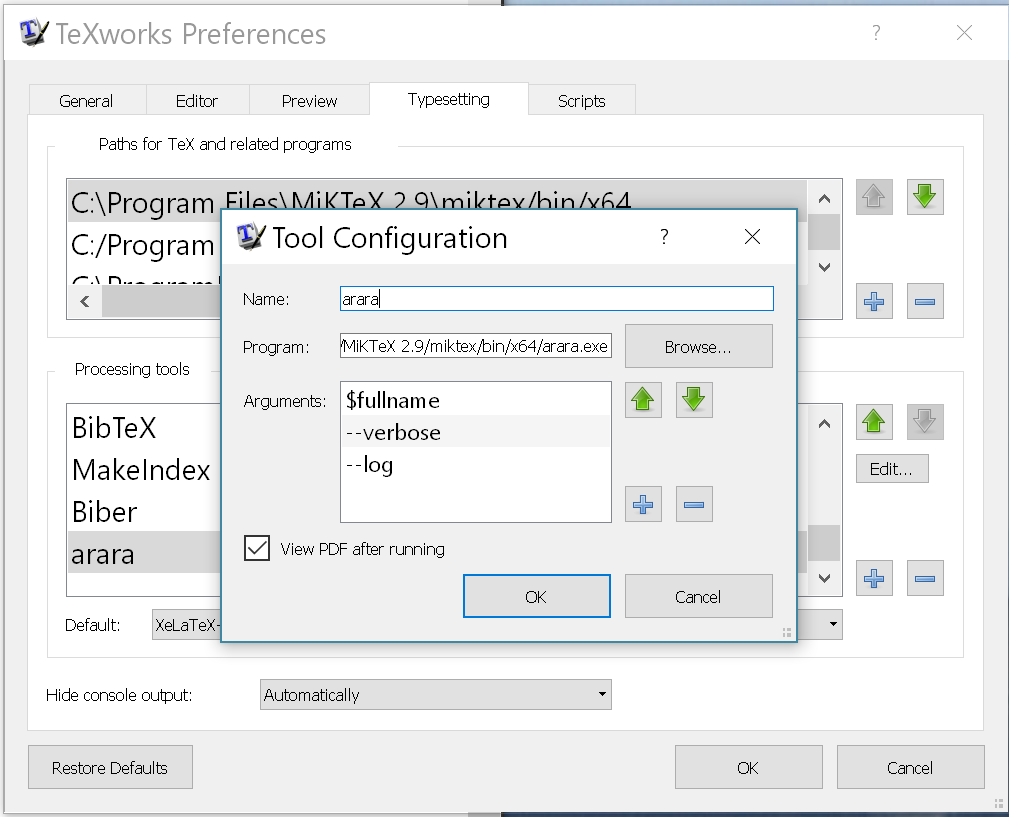
\includegraphics[scale=0.5]{../fig/arara.png}
\caption{Configuring {\TeX}works for \texttt{arara}.}
\label{fig:arara}
\end{figure}

%------------------------------------------------------------------------------
% \begingroup  % Temporarily disable \clearpage to show both lists on one page
%   %\let\clearpage\relax    % http://tex.stackexchange.com/a/14511/104449
%   \renewcommand{\listtheoremname}{List of definitions}
%   \textsf{\listoftheorems[ignoreall, show={definition}]}
% \endgroup
%-------------------------------------------------------------------------------
% \renewcommand{\listfigurename}{Figures}
% \addcontentsline{toc}{chapter}{\listfigurename}
% \begingroup
% \let\onecolumn\twocolumn
% \sffamily
% \listoffigures
% \rmfamily
% \endgroup
%-------------------------------------------------------------------------------
% \renewcommand{\lstlistlistingname}{Code samples}
% \addcontentsline{toc}{chapter}{\lstlistlistingname}
% \begingroup
% \let\onecolumn\twocolumn
% \sffamily
% \lstlistoflistings
% \rmfamily
% \endgroup
%-------------------------------------------------------------------------------
% \renewcommand{\listtheoremname}{Examples}
% \addcontentsline{toc}{chapter}{\lstlistlistingname}
% \begingroup
% \let\onecolumn\twocolumn
% \sffamily
% \listoftheorems
% \rmfamily
% \endgroup
%-------------------------------------------------------------------------------
% \newglossarystyle{mystyle}{%
%  \glossarystyle{altlist}%
%  \renewcommand*{\glossaryentryfield}[5]{%
%    \item[\glsentryitem{##1}\glstarget{##1}{##2}]%
%       :\hspace{1em}##3\glspostdescription\space ##5}%
% }
% \printglossary[title=Glossary,toctitle=Glossary]
%-------------------------------------------------------------------------------
\printbibliography[heading=bibintoc, title={References}]
%-------------------------------------------------------------------------------
% \printindex
%-------------------------------------------------------------------------------

\end{document}
